% Créé par Martin Bodin (2011).
% Document sous licence CC BY-NC-SA

% Créé par Martin Bodin (2011).
% Document sous licence CC BY-NC-SA

\documentclass{article}
%\documentclass{scrartcl}

\usepackage{ifxetex}
\ifxetex
\usepackage{xunicode,fontspec,xltxtra}
\else
\usepackage[utf8x]{inputenc}
\usepackage[T1]{fontenc}
\usepackage{amsmath, amsthm}
\usepackage{amsfonts, amssymb}
\fi

\usepackage[francais]{babel}
\usepackage{lmodern}
\usepackage{stmaryrd}
\usepackage{graphicx}
\usepackage[nottoc, notlof, notlot]{tocbibind}
\usepackage[dvipsnames]{pstricks}
\usepackage{pst-circ, pst-plot, pstricks-add}
\usepackage{array}
\usepackage{url}
\usepackage{verse}
\usepackage[colorlinks,linkcolor=black]{hyperref}
\usepackage{ifthen}
\usepackage{longtable, rotating}
%\usepackage{fancyhdr}
\usepackage{fancybox, framed}
\usepackage{textcomp}
\usepackage{marvosym}
%\usepackage{bbding}
%\usepackage{a4wide}
\usepackage{geometry}
%\usepackage{soul}
\usepackage{lettrine}
%\usepackage{yfonts}
\usepackage{oldgerm}
\usepackage{enumerate}
\usepackage{tikz}
\usepackage{dictsym}
\usepackage{pifont}

\ifxetex
\newfontfamily\timesfont[Ligatures=TeX]{Times New Roman}
\setmainfont[Mapping=tex-text, Ligatures={Contextual, Common, Historical, Rare, Discretionary}, Numbers={OldStyle}]{Linux Libertine O}
\fi

%\newcommand{\enluminure}[2]{\lettrine[lines=3]{\small \initfamily #1}{#2}}

\usetikzlibrary{trees}
\usetikzlibrary{arrows,shapes,automata,petri}
\usetikzlibrary{fit}
\usetikzlibrary{calc,decorations.pathmorphing,patterns}


\geometry{
	includeheadfoot,
	margin = 2.54cm,
	top = 1.5cm,
	bottom = 1.5cm
}

\newcommand{\ds}{\displaystyle}

\renewcommand{\ge}{\geqslant}
\renewcommand{\le}{\leqslant}
\renewcommand{\preceq}{\preccurlyeq}
\renewcommand{\succeq}{\succcurlyeq}

\newcommand{\Numero}{\No}
\newcommand{\numero}{\no}

\newcommand{\fixme}{\textbf{FIXME}}

\makeatletter

\newcommand{\defineNewPlayer}[2]{
	\@namedef{couleur#1}{#2}
}

\newcommand{\getPlayerColor}[1]{%
	\@nameuse{couleur#1}%
}

\makeatother

% Des commandes pratiques pour générer le document.
\newcommand{\player}[2]{%
	\ifthenelse{\equal{\forplayer}{y}}{%
		\ifthenelse{\equal{\theplayer}{#1}}%
		{#2}{}%
	}{\begin{barv}[\getPlayerColor{#1}]{2pt}{10pt}#2\end{barv}}%
}
\newcommand{\mj}[1]{%
	\ifthenelse{\equal{\forplayer}{n}}{#1}{}%
}
% Ici suit une commande plus complexe, car plus générale.
\makeatletter

\newcommand{\@beginColor}[3][black]{%
	\ifthenelse{\equal{\forplayer}{n}}{%
		\begin{barv}[#1]{#2}{#3}%
	}{}%
}

\newcommand{\@endColor}{%
	\ifthenelse{\equal{\forplayer}{n}}{%
		\end{barv}%
	}{}%
}


\newcommand{\ignore}[1]{}
\newcommand{\@ident}[3]{%
%	\ifthenelse{\equal{\manyColored}{y}}{#1}{%
%		\marginpar{%
%			#1%
%			\vspace{2cm}%
%			#2%
%		}%
%	}%
	#1%
	\ifthenelse{\equal{\forplayer}{n}}{\@beginColor{0pt}{10pt}}{}%
	#3%
	\ifthenelse{\equal{\forplayer}{n}}{\@endColor}{}%
	#2%
%	\ifthenelse{\equal{\manyColored}{y}}{#2}{%
%		\marginpar{%
%			#1%
%			\vspace{5pt}%
%			#2%
%		}%
%	}%
}

\def\@ouverture#1#2{%
\ifthenelse{\equal{\forplayer}{y}}{}{%
\ifthenelse{\equal{\manyColored}{y}}{\@beginColor[#1]{1pt}{0pt}}{%
\hspace{-1cm}\hspace{-#2mm}\parbox[c][1pt][t]{0pt}{
\begin{tikzpicture}
	\node (a) {};
	\node (b) [right of = a, node distance = 16cm] {};
	\node (c) [below of = a, node distance = 2cm] {};
	\draw [very thick, color = #1] (a.center) -- (b);
	\draw [very thick, color = #1] (a.center) -- (c);
\end{tikzpicture}
}\vspace{-3.2mm}\par%
}%
}%
}
\def\@fermeture#1#2{%
\ifthenelse{\equal{\forplayer}{y}}{}{%
\ifthenelse{\equal{\manyColored}{y}}{\@endColor}{%
\hspace{-1cm}\hspace{-#2mm}\parbox[c][1pt][b]{0pt}{
\begin{tikzpicture}
	\node (a) {};
	\node (b) [right of = a, node distance = 16cm] {};
	\node (c) [above of = a, node distance = 1cm] {};
	\draw [very thick, color = #1] (a.center) -- (b);
	\draw [very thick, color = #1, dashed] (a.center) -- (c);
\end{tikzpicture}
}\vspace{-3.2mm}\par%
}%
}%
}

\def\players@parse#1#2[#3][#4]{%
% #1 :  Suite de \@ouverture
% #2 :  Suite de \@fermeture
% #3 :  Commande à appeler dans le cas d’une réponse négative (≃ réponse précédente).
% #4 :  Argument (sous forme de numéro de joueur) lu actuellement.
	\ifthenelse{\equal{\theplayer}{#4}}{%
		\players@yes{\@ouverture{\getPlayerColor{#4}}{#4}#1}{#2\@fermeture{\getPlayerColor{#4}}{#4}}%
	}{%
		#3{\@ouverture{\getPlayerColor{#4}}{#4}#1}{#2\@fermeture{\getPlayerColor{#4}}{#4}}%
	}%
}

\def\players@no#1#2{%
	\@ifnextchar[{\players@parse{#1}{#2}[\players@no]}{\ignore}%
}

\def\players@yes#1#2{%
	\@ifnextchar[{\players@parse{#1}{#2}[\players@yes]}{\@ident{#1}{#2}}%
}

\def\players{%
	\ifthenelse{\equal{\forplayer}{y}}{%
		\players@no{}{}%
	}{%
		\players@yes{}{}%
	}%
}

% \players{…} est quasi-équivalent à \mj{…}.
% \players[i]{…} est équivalent à \player{i}{…}
% \players[i][j][k]{…} va créer du contenu uniquement pour les joueurs i, j et k (et les MJ bien sûr).

\makeatother
%\fixme :  Ces commandes posent des problèmes pour toutes les sections, footnote, etc. :S

\newcommand{\colorForMJ}[2]{%
	\ifthenelse{\equal{\forplayer}{y}}{#2}{%
		\textcolor{\getPlayerColor{#1}}{#2}%
	}%
}
\newcommand{\synopsisPerso}[3]{%
\paragraph{}{
\textbf{\fcolorbox{\getPlayerColor{#1}}{white}{#2}}\hspace{10pt}%
{#3}}%
}

\newenvironment{changemargin}[2]{\begin{list}{}{%
\setlength{\topsep}{0pt}%
\setlength{\leftmargin}{0pt}%
\setlength{\rightmargin}{0pt}%
\setlength{\listparindent}{\parindent}%
\setlength{\itemindent}{\parindent}%
\setlength{\parsep}{0pt plus 1pt}%
\addtolength{\leftmargin}{#1}%
\addtolength{\rightmargin}{#2}%
}\item }{\end{list}}
\reversemarginpar
%\pagestyle{fancy}
%\fancyhf{}
%\renewcommand{\headrulewidth}{0pt}
%\lhead{}
%\lfoot{}

\makeatletter
\newenvironment{barv}[3][black]{%
% #2 largeur du trait
% #3 distance entre le trait et le texte
	\def\FrameCommand{{\color{#1}\vrule width #2}
	\hspace{#3}}%
	\MakeFramed {\advance \hsize -\width \FrameRestore }%
}{%
    \endMakeFramed%
}
\makeatother


\definecolor{LightButter}{rgb}{0.98,0.91,0.31}
\definecolor{LightOrange}{rgb}{0.98,0.68,0.24}
\definecolor{LightChocolate}{rgb}{0.91,0.72,0.43}
\definecolor{LightChameleon}{rgb}{0.54,0.88,0.20}
\definecolor{LightSkyBlue}{rgb}{0.45,0.62,0.81}
\definecolor{LightPlum}{rgb}{0.68,0.50,0.66}
\definecolor{LightScarletRed}{rgb}{0.93,0.16,0.16}
\definecolor{Butter}{rgb}{0.93,0.86,0.25}
\definecolor{Orange}{rgb}{0.96,0.47,0.00}
\definecolor{Chocolate}{rgb}{0.75,0.49,0.07}
\definecolor{Chameleon}{rgb}{0.45,0.82,0.09}
\definecolor{SkyBlue}{rgb}{0.20,0.39,0.64}
\definecolor{Plum}{rgb}{0.46,0.31,0.48}
\definecolor{ScarletRed}{rgb}{0.80,0.00,0.00}
\definecolor{DarkButter}{rgb}{0.77,0.62,0.00}
\definecolor{DarkOrange}{rgb}{0.80,0.36,0.00}
\definecolor{DarkChocolate}{rgb}{0.56,0.35,0.01}
\definecolor{DarkChameleon}{rgb}{0.30,0.60,0.02}
\definecolor{DarkSkyBlue}{rgb}{0.12,0.29,0.53}
\definecolor{DarkPlum}{rgb}{0.36,0.21,0.40}
\definecolor{DarkScarletRed}{rgb}{0.64,0.00,0.00}
\definecolor{Aluminium1}{rgb}{0.93,0.93,0.92}
\definecolor{Aluminium2}{rgb}{0.82,0.84,0.81}
\definecolor{Aluminium3}{rgb}{0.73,0.74,0.71}
\definecolor{Aluminium4}{rgb}{0.53,0.54,0.52}
\definecolor{Aluminium5}{rgb}{0.33,0.34,0.32}
\definecolor{Aluminium6}{rgb}{0.18,0.20,0.21}

\pgfdeclarelayer{foreground} 
\pgfdeclarelayer{background} 
\pgfsetlayers{background,main,foreground} 



\newcommand{\forplayer}{n} % or y
\newcommand{\theplayer}{13} % if \equal{\forplayer}{y}, then it represents the number of this player.
\newcommand{\manyColored}{n} % If seems that too many nested “barv” environments make LaTeX complains.

\defineNewPlayer{1}{MidnightBlue} % Le Roi
\defineNewPlayer{2}{Cyan} % La Princesse
\defineNewPlayer{3}{Gray} % La Reine
\defineNewPlayer{4}{OliveGreen} % Le Cavalier
\defineNewPlayer{5}{Red} % Le Chevalier
\defineNewPlayer{6}{YellowOrange} % Le Fol
\defineNewPlayer{7}{Sepia} % Le gardien
\defineNewPlayer{8}{Rhodamine} % Le Sage
\defineNewPlayer{9}{Violet} % La Voyante
\defineNewPlayer{10}{Plum} % L’inconnu
\defineNewPlayer{11}{LimeGreen} % L’Inventeur
\defineNewPlayer{12}{Salmon} % Le Lapin
\defineNewPlayer{13}{BlueViolet} % Armand

\newcommand{\cartetarot}[5]{\includegraphics[width=1.3cm]{images/tarot/#1.jpg} & \parbox[s]{1.9cm}{#2} & \rotatebox{-90}{\small #3} & #4 & #5 \\\hline}

\newcommand{\citations}[1]{
\paragraph{Phrases de combats}{
Les phrases de combats qui suivent sont les phrases sacrées de votre famille, vos phrases de duel favorites, ou autre.
Dans tous les cas, le fait est que vous les connaissez par cœur et que vous les utilisez dans tous vos combats d’épées.

Apprenez les~:  le jour de la murder, vous en aurez besoin si jamais vous vous engagez dans un duel à l’épée\footnote{
Ou tout autre duel d’ailleurs~!
}~!
Le but\footnote{
Ne vous inquiétez pas si cela paraît vous vague, c’est tout simplement parce qu’il existe plusieurs épreuves possibles (choisies par le Roi) et qu’elles seront décrites le moment venu.
Globalement, ce seront des épreuves où le but sera de ridiculiser l’autre avec des contraintes plus ou moins fortes sur ce que vous pouvez dire.
} sera pour votre adversaire d’y répondre de la meilleure façon possible (exemple typique\footnote{Tiré de \textsc{Monkey Island}.}~:  à «~Tous tes mots sont idiots.~», vous pouvez répondre «~J'essayais de me mettre à ton niveau.~» — remarquez que la complexité des répliques dépendent de la complexité du personnage~: préparez vous au pire si vous redoutez votre adversaire~!), mais si vous le prononcez mal, il n’en aura même pas besoin~!

Voici donc vos fameuses phrases de combats~:
\begin{itemize}
	#1
\end{itemize}
}
}

\title{Bien longtemps après Alice}
\author{Martin \textsc{Bodin}}
\date{}

\begin{document}

\maketitle

\tableofcontents

\vfill

\hfill
Scénario créé par Martin \textsc{Bodin}, sous licence CC BY-NC-SA.
\hfill

\includegraphics[width = 20pt]{images/licence/cc-by.png}

\includegraphics[width = 20pt]{images/licence/cc-nc.png}

\includegraphics[width = 20pt]{images/licence/cc-sa.png}

\newpage

\section{À propos de l’univers}

J’aimerais tout d’abord attirer votre attention sur le fait que nous sommes dans un conte.
Vous remarquerez donc que la plupart des personnages n’ont pas de nom, mais plutôt un rôle (le Roi, le Sage, etc.).
J’ai volontairement mélangé des termes issus des jeux de cartes, des échecs, d’\textsc{Alice au Pays des merveilles} et mixé des idées venant des personnages de \textsc{De Capes et de Crocs} et de \textsc{Monkey Island}~:  je ne cherche pas à faire quelque chose de cohérent, juste quelque chose de rigolo.
J’espère que ce scénario vous plaira tout autant que moi~!

Globalement, tout se passe dans le Pays des merveilles, bien après (si la notion d’«~après~» a réellement un sens dans cet univers) le retour d’Alice pour affronter la Reine de Cœur.
Le Pays des merveilles a cessé d’être le rêve d’Alice et il commence à s’effacer à certains endroits.
Mais bon, les gens essaient de vivre malgré la menace de s’effacer à leur tour…
Dans ses derniers rêves, Alice — qui a beaucoup grandi — a rendu ce monde plus «~sérieux~».
Des villages peuplés d’humains pas vraiment aussi fous que le Chapelier sont apparus et ont remplacés la plupart des cartes.
\player{3}{Alice s’est aussi désillusionné quant à la Reine blanche qui va devenir avide de pouvoir par la suite…\footnote{
N’oublions pas que la Reine blanche est le miroir de la Reine rouge…  Maintenant, les rôles sont justes plus ou moins inversés.}}

La Reine blanche a gardé la partie «~traditionnelle~» du royaume, composée de la plupart des créatures fantastiques (au hasard, les cartes).
L’autre partie s’est transformée en un nouveau royaume~:  le royaume de Coupes.

\paragraph{Synopsis}
{
Le Roi de Coupes cherche un mari pour la princesse~!
La grande nouvelle s’est répandue en flèche dans tout le royaume~:  le Roi organise un concours artistique, dont le gagnant obtiendra la main de sa fille.

Les enjeux sont de taille~:  depuis que le monde du rêve perd de sa substance, celui-ci devient de moins en moins utopique, et beaucoup de gens ont peur que tout cela empire.
Se marier avec la Princesse~!  Devenir Prince~!
Voilà de quoi être à l’abri d’un tel effondrement tant que le Pays des merveilles existe encore.
}

\section{Présentation du Royaume de Coupes}

\players[1][2][5][7][8][9][10][11][12][13]{
\subsection{Le Royaume}
}

C’est un royaume très jeune, issu d’une séparation (dont la cause n’est pas très claire) d’une province du Royaume blanc (gouverné par la Reine blanche).
Le symbole du Royaume est une coupe sur fond étoilé~:
\begin{center}

\includegraphics[width=5cm]{images/Royaume_de_Coupes_logo.png}
\end{center}

Les relations avec les royaumes voisins (et en particulier le Royaume blanc) ne sont pas spécialement tendues et la Reine blanche est accueillie tout naturellement ici sans que sa visite ne soit considérée comme hostile.

Voici une carte du Pays des merveilles.
Les frontières du Royaume de Coupes sont en bleu, celles de l’ancien Royaume de Cœur en rouge et celles du Royaume blanc à son apogée (c’est à dire lorsqu’il contenait encore le Royaume de Coupes) en blanc.
\begin{center}
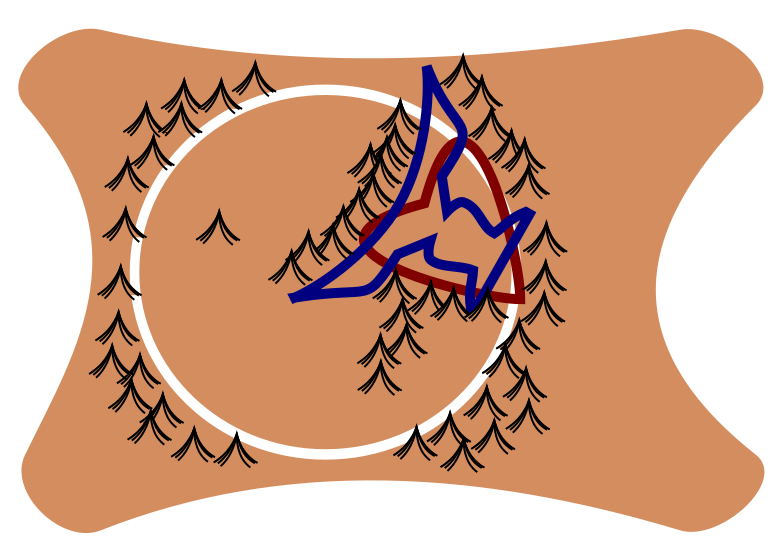
\includegraphics[height=10cm]{images/carte.png}
\end{center}

\players[1][2][5][7][8][9][10][11][13]{
Le Royaume de Coupes possède de nombreuses traditions.
En particulier, il a un système de duels organisés relativement complexe.

Lorsque deux personnes veulent se battre en duel, elles demandent en effet à la cour de les aider dans leur différent.
Le Roi va alors choisir une épreuve et la cour va arbitrer les duellistes.

Le Roi ne choisit pas forcément des épreuves mortelles (c’est même assez rare)~:  par exemple la \textit{Rixme} est un duel de mots souvent choisit par le Roi à cause de son côté non violent et plaisant.

\subsection{Les différentes personnes qui le composent}
Voici les personnes\footnote{
Plus la tour, je sais…
} principales qui composent le royaume.
Il y a bien entendu d’autres personnes, mais s’ils ne sont pas ici, il est probable que vous ne connaissiez que de nom.
En cas de doute pendant la partie, n’hésitez pas à demander aux maîtres du jeu des informations que votre personnage pourrait connaître.

\paragraph{Le Roi}{
C’est un Roi mécène qui vit pour la poésie, le symbole du Royaume.
C’est lui qui choisit l’épreuve lors d’un duel et qui l’arbitre la plupart du temps.
}

\paragraph{Le Sage}{
Conseiller du Roi, ses conseils d’ancien sont assez réputés.
Il arbitrera parfois sous ordre du Roi certaines joutes verbales.
Il accepte parfois de conseiller d’autres personnes que le Roi (qui ne proviennent pas forcément de la cour).
Ses conseils sont assez réputés pour leur justesse et leur pragmatisme.
}

\paragraph{L’Inventeur}{
Autre conseiller du Roi.
C’est aussi lui le poète officiel du Roi.
}

\paragraph{Le Chevalier de Coupes}{
C’est le maître d’arme du Royaume.
Il est très réputé pour cela.
}

\paragraph{La Tour}{
C’est la tour sacrée qui contient en plus de la bibliothèque royale toutes les œuvres d’arts du Roi.
Elle est gardée par le fameux Gardien de la Tour.
}

\paragraph{La Princesse}{
Très belle.
C’est aussi elle qui succédera au Roi.
}

\paragraph{La Voyante}{
Ses talents sont très réputés de par le Royaume.
}
}

\player{8}{
\section{Préceptes principaux du jeu de Go.}

\player{8}{
Ton personnage utilise tous ces préceptes pour les appliquer dans la vie de tous les jours.
Son premier réflexe lorsqu’on lui énonce un précepte est de le dessiner sur un Goban par des pierres de Go, puis d’analyser (on parlera de «~lire~» le Goban) la situation en jouant un peu.
}

\begin{enumerate}
\item La gourmandise n’apporte pas la victoire.
\item Pénétrer la sphère gentiment et facilement.
\item Si vous attaquez votre adversaire, surveillez vos arrières.
\item Abandonnez le menu fretin ; combattez pour l’initiative.
\item Laissez tomber le petit, accrochez-vous au gros.
\item Si vous êtes en danger, abandonnez quelque chose.
\item Soyez prudent, ne vadrouillez pas de ci de là sur tout le goban.
\item Rendre coup pour coup si nécessaire.
\item Si votre adversaire est fort, protégez-vous.
\item Si votre groupe est isolé au centre d'une influence adverse, choisissez la voie pacifique.
\end{enumerate}
}

\players[6][9][10]{
\section{Signification des arcanes majeurs}

Et oui, les cartes du tarot ne servent pas qu’à jouer~:  elles servent surtout à prédire l’avenir.
Il existe de nombreuses façons de prédire l’avenir, avec ou sans les Arcanes mineurs par exemple.
Dans tous les cas, les cartes les plus importantes sont les \emph{Arcanes majeurs}\footnote{On les appelle les atouts dans l’actuel tarot.}, chacune ayant deux interprétations majeures suivant qu’elle ai été tirée à l’endroit ou à l’envers (du point de vue du médium).

Je précise aussi que les autres cartes (les \emph{Arcanes mineurs}) du jeu de Tarot sont bien entendu aussi présentes dans le Tarot de Marseille (car c’est de celui-ci que l’on parle ici), mais elles sont moins utilisées pour la prédiction de l’avenir.
Juste pour la culture, on ne parle pas de Piques, Trèfles, Cœur et Carreaux dans ce Tarot, mais d’Épées, de Batons, de Coupes et de Deniers (dénominations qui sont d’ailleurs restées dans plusieurs pays, l’\textsc{Espagne} par exemple).

\player{6}{
En tant que compteur, tu les utilises surtout pour leurs valeurs et par commodité pour créer tes chants.
Bien entendu, en tant que philosophe, tu te moques bien de ces croyances stupides.
Cependant il faut le dire, les symboles du jeu de tarot sont \emph{beaux} et tu aimes les utiliser pour ça.

Voici la signification des différents Arcanes majeurs.
}

\player{10}{
Voici la signification des différents Arcanes majeurs.
}

\player{9}{
\subsection{Comment prédire l’avenir}

La méthode la plus simple est celle du \emph{tirage en croix}.
Elle consiste à tirer quatre ou cinq cartes et à les placer en croix, l’axe horizontale représentant les forces actuelles en présence et l’axe verticale l’enchaînement dans le temps.

Comme toujours en cartomancie, le client pose une question.
Puis on bat les cartes (seulement les Arcanes majeurs), puis les coupe.

La première carte tirée est placée à gauche.
Elle représente la personne qui pose la question ou le sujet de la question suivant le cas.

La seconde est placée à droite.
Elle représente les forces qui vont empêcher le sujet de la question d’agir dans le sens de sa volonté.
On peut voir ces deux premières cartes comme un combat bon/mal.

La troisième est placée en haut.
Elle représente le présent ou le futur immédiat.

La quatrième carte est placée en bas.
C’est la carte la plus importante avec la première puisqu’elle indique ce qui va se passer ensuite.

Enfin, lorsqu’un doute sur l’interprétation subsiste, il est possible de tirer une cinquième carte pour la mettre au centre.
Cette carte a moins d’importance que toutes les autres, mais elle permet de nuancer la réponse.
Elle n’est en aucun cas indispensable.

Il est à noter que plus la question est imprécise, plus la réponse doit l’être.
Si la question est «~Quel est mon avenir~?~», la réponse sera vague au possible.
Si la question est «~Est-ce que j’arriverais à convaincre telle personne de faire telle action~?~», la réponse — bien que souvent très nuancée — sera relativement précise.

\subsection{Signification des Arcanes}

Voici la signification des Arcanes majeurs.
Attention, ne pas oublier en tirant que l’orientation d’une carte a une signification.
}

%\newpage
%\begin{turn}{90}
%\enlargethispage{3cm}
%\begin{minipage}{20cm}
\setlongtables
\hspace{-5cm}\begin{longtable}{|m{1.35cm}|m{1.9cm}|m{0.5cm}|m{4.5cm}|m{4.5cm}|}
\hline \multicolumn{5}{|c|}{Signification des Arcanes majeurs}
\\ \hline Image & Nom & {\small{}Var-iante} & Interprétation endroit & Interprétation envers\\\hline
\endfirsthead
\hline Image & Nom & {\small{}Var-iante} & Interprétation endroit & Interprétation envers\\\hline
\endhead
\endfoot
\cartetarot{LeBateleur}{I \\ Le Bateleur}{Le Magicien}{Activité créatrice, initiative, présence d'esprit, émancipation. Art de convaincre. Choses mises en action, qui bougent.}{Absence de scrupules. Personnage arriviste, intrigant, escroc. Individu utilisant l'agitation, la tromperie. Volonté faible.}
\cartetarot{LaPapesse}{II \\ la Papesse}{}{Inertie, méditation. Réserve, discrétion, attente confiante, patience, résignation, bonté, bienveillance, clairvoyance.}{Hypocrisie, dissimulation, intentions cachées. Inaction, paresse. Immoralité, rancune.}
\cartetarot{LImperatrice}{III \\ L’Impératrice}{}{Réflexion, observation. Idée dont la réalisation est à poursuivre. Savoir, intelligence. Abondance, élégance, charme.}{Vanité, prétention, dédain. Sensibilité à la flatterie, frivolité, luxe, séduction, coquetterie.}
\cartetarot{LEmpereur}{IV \\ L’Empereur}{}{Action visant à concrétiser. Volonté inébranlable. Concentration. Rigueur. Protecteur puissant, mais contrôlant.}{Entêtement, parti-pris hostile. Gros risque d'échec. Tyrannie, absolutisme.}
\cartetarot{LePape}{V \\ Le Pape}{}{Méditer pour comprendre. Guide, conseils, bienveillance. Silence, discrétion, modestie, patience, respect. Convenances.}{Intentions cachées, intolérance, rancune. Inertie, paresse, fanatisme. Conseiller sans aucun sens pratique, moraliste étroit.}
\cartetarot{LesAmoureux}{VI \\ Les Amoureux}{L’amoureux}{Libre arbitre. Choix, vœux, souhaits, aspirations. Délibérations, responsabilités. Amour.}{Perplexité, promesses et désirs irréalisés. Tentation. Épreuve à subir, doute, incertitude.}
\cartetarot{LeChariot}{VII \\ Le Chariot}{Le Char}{Succès légitime, ambition, progrès, intelligence et tact. Direction compétente, qualités de chef.}{Oppositions, ambitions injustifiées, situation usurpée. Manque de talent, de tact. Incompétence, opportunisme. Surmenage.}
\cartetarot{LaJustice}{VIII \\ La Justice}{}{Indépendance d'esprit, impartialité, honnêteté, discipline. Règle de conduite. Conséquences inéluctables de toute action.}{Paperasseries, procès. Manque d'initiative, obéissance. Routine, fonctionnarisme.}
\cartetarot{LHermite}{IX \\ L’Hermite}{Le Dragon}{Recueillement. Sagesse intérieure, discrétion, isolement, étude, expérience, tradition, patrimoine. Sage détaché du monde. Mage ou occultiste.}{Isolement forcé. Caractère méfiant, songeur. Découragement, tristesse, timidité, mutisme. Célibat, solitude. Conspirateur.}
\cartetarot{LaRouedeFortune}{X \\ La Roue De La Fortune}{}{Initiative heureuse, donner foi à son intuition. Réussite fortuite, spontanéité, bonne humeur.}{Abandon au hasard, insécurité, imprévoyance, insouciance. Situation instable, malchance, imprévus, manque de sérieux.}
\cartetarot{LaForce}{XI \\ La Force}{}{Force morale s'imposant d'elle-même à la force brutale. Âme forte, maîtrise de soi-même. Courage.}{Caractère vif, téméraire, violent. Impatience, colère, insensibilité, cruauté, tyrannie. Lutte, guerre, discorde.}
\cartetarot{LePendu}{XII \\ Le Pendu}{}{Sacrifice volontaire au bénéfice d'une cause élevée. Oubli total de soi-même, désintéressement absolu au matérialisme. Illuminé.}{Rêveur, utopiste. Enthousiasme nourri d'illusions. Amour non partagé. Projets non réalisés. Pertes.}
\cartetarot{LaMort}{XIII \\ L’Arcane sans nom}{La Mort}{Évolution, pouvoir transformateur capable de régénérer. Esprit de progrès, d'avancement. Désillusion.}{Transformation radicale et subite. Fin nécessaire. Fatalité. Pessimisme, tristesse, deuils.}
\cartetarot{LaTemperance}{XIV \\ La Tempérance}{}{Alchimie, régénération, miracles. Indifférence aux mesquineries de la vie. Facilité d'adaptation, bonne santé.}{Impressionnabilité, nature instable et changeante. Laisser-aller. Passivité, indifférence, imprévoyance.}
\cartetarot{LeDiable}{XV \\ Le Diable}{}{Instinct, impulsivité. Sorcellerie, envoûtement, fascination. Domination des masses. Excès.}{Excès et immodération sous toutes ses formes, déchéance, perversion, animalité, cupidité, égoïsme… Déséquilibre, désordre, machinations.}
\cartetarot{LaTour}{XVI \\ La Maison-Dieu}{La Tour}{Avidité d'acquérir, égoïsme, ambitions et appétits insatiables. Volonté d’aller contre la nature.}{Chaos total. Échec mérité et prévisible de toute entreprise insensée. Désorganisation, maladie.}
\cartetarot{LEtoile}{XVII \\ L’Étoile}{}{Le monde de la nuit et ses mystères, le sommeil et ses révélations. Idéal que la Vie tend à réaliser. Espérance, bonne humeur}{Perte d'espoir. Naïveté, ignorance. Séduction, sensualité, rêverie. Impudeur. Curiosité indiscrète.}
\cartetarot{LaLune}{XVIII \\ La Lune}{}{Imagination, sensibilité en éveil favorisant les arts. Chemin pénible mais nécessaire. Lubie, imagination, extravagances.}{Illusions, mensonges, égarement, fausses suppositions. Recherches longues et difficiles, travail imposé, pauvreté, misère. Fausse sécurité, pièges.}
\cartetarot{LeSoleil}{XIX \\ Le Soleil}{}{Discernement, illumination géniale, clarté de jugement. Fraternité, harmonie, grandeur d'âme, paix, amitié, affection. Gloire. Talents artistiques ou littéraires.}{Désir de paraître, éblouissement, vanité. Bluff, décors prestigieux. Susceptibilité. Amour-propre démesuré.}
\cartetarot{LeJugement}{XX \\ Le Jugement}{}{Possibilités nouvelles, fin d'un cycle difficile. Réparation de torts subis, libération, guérison, jugement équitable. Renommée. Inspiration.}{Peur du changement, indécision. Enivrement spirituel. Surexcitation (naturelle ou artificielle), manque de pondération.}
\cartetarot{LeMonde}{XXI \\ Le Monde}{}{Accomplissement, succès. Harmonie et équilibre. Circonstances très favorables. Joie, perfection.}{Retard. Obstacle extérieur insurmontable, revers de fortune. Distraction.}
\cartetarot{LeMat}{0 \\ Le Mat}{Le Fou, L’Alfil}{Intuition, optimisme, innocence. Besoin de liberté et d'indépendance. Pensées et actions dépassant souvent l'entendement humain. Originalité, Créativité. Nouveau départ.}{Extravagance, risque de folie. Incapacité de raisonner par soi-même, de se diriger. Aveugle inconscient entraîné à sa perte, déséquilibré influençable, insensé s'abandonnant à ses lubies.}
\end{longtable}
%\end{minipage}
%\end{turn}
}

\mj{
\newpage

\section{Présentation globale des personnages}

\synopsisPerso{1}{Le Roi de Coupes}
{
Ce personnage est un peu à part puisqu’il va faire partie des juges lorsqu’un combat entre deux personnages aura lieu, un peu comme un maître du jeu temporaire qui ne connaîtrait pas le scénario.
C’est lui qui choisira l’épreuve parmi un certain choix donné par les véritables maîtres du jeu (voir section~\ref{sec:epreuves}).

C’est un roi qui se veut poète, tel le Roi sélénite dans \textsc{De Capes et de Crocs}.
Très grand mécène, plusieurs artistes se pressent dans sa cour, et il n’hésite pas à s’entretenir avec eux pour des affaires politiques.
Il rêve d’un monde où tout est harmonie et poésie.

Le fait que son monde semble sombrer dans un néant de manière plus ou moins inéluctable le fait craindre que les divertissements en tous genres soient supprimés.
Déjà les premiers problèmes de famine pourraient bientôt apparaître (ce qui ne se sera jamais fait voir au Pays des merveilles~!) et il craint que cela empêche les gens de penser à autre chose qu’aux besoins vitaux.
Il n’y a pas de monnaie au Pays des merveilles, mais s’il y en avait une, ce serait des poèmes~:  jamais ce Roi ne pourrait accepter autre chose comme objet ayant de la valeur en soi.
}

\synopsisPerso{2}{La Princesse de Coupes}
{
Fille du Roi, très cultivée et très charmante.
Mais derrière ses apparences de fille parfaite, se cache un personnage qui rêve d’aventure.
Son père cherche à lui trouver un mari, mais elle ne veut ni se marier ni consacrer sa vie à la poésie.
Elle rêve de voyager à travers le monde et admire le Chevalier de Coupes pour cela… d’ailleurs, courtiser le Chevalier paraît être la meilleure solution pour s’échapper de son père.
}

\synopsisPerso{3}{La Reine blanche}
{
Elle est jalouse du royaume de Coupes.
C’est pourtant elle qui s’était présentée comme sage et douce lors du dernier passage important d’Alice, mais entre-temps, les rêves d’Alice l’ont rendu plus «~réaliste~» et avide de pouvoir.

Elle dirige actuellement le «~Royaume blanc~» qui contient plus ou moins tout les êtres fantastiques restant au Pays des merveilles.

Malheureusement, avec l’Effondrement, beaucoup d’entre eux ont tout simplement disparus~:  les cartes sont devenues beaucoup plus rares et ne peuvent plus partir du Royaume blanc, le Chat du Cheschire a disparu pour de bon, le prêtre mouton se met à bêler de plus en plus, etc.
Elle va alors chercher à redevenir la véritable reine de tout le Pays, en pensant que cela va rétablir l’utopie du rêve.

Au début du scénario, elle arrive à l’improviste au royaume de Coupes — sans demander particulièrement à voir le Roi — et va tenter de le renverser sans que personne ne la soupçonne pendant la partie.
Le fait qu’elle débarque comme cela ne gène pas spécialement les gens, ses visites étant régulières au royaume de Coupes.

Un détail qui peut avoir son importance est que la notion de temps a peu d’importance dans cet univers, ce qui va impliquer par exemple que malgré les quelques jours où la Reine se trouve au Royaume blanc, il est tout à fait possible d’imaginer que plusieurs années se soient passées dans le Royaume blanc~!
Ce détail peut-être utilisé pour qu’un tirage de la Voyante ou une phrase de l’Inconnu (voir plus loin) se réalise…
}

\synopsisPerso{4}{Le Cavalier}
{
Exemple typique du personnage qui voyage et qui cherche à avoir la main de la Princesse.
Malheureusement, ses qualités artistiques ne sont pas vraiment à la hauteur pour ça…
Il a cherché plusieurs moyens de détourner ce problème.
Même si la triche n’est pas vraiment dans ses habitudes, il n’hésitera pas longtemps à voler un poème (typiquement à l’Inventeur) et se l’approprier.

Il est très jeune et a passé une bonne partie de sa vie solitaire à arpenter les champs.
Le Chevalier lui a appris il y a bien longtemps cette botte secrète et imbattable qu’est la «~botte de Jamais~», mais il l’utilise très peu puisqu’elle n’est imbattable que lorsque les adversaires sont à force égale dans un duel d’honneur, ce qui est rarement le cas en campagne…
}

\synopsisPerso{5}{Le Chevalier de Coupes}
{
Il a grandi et vécu toute son enfance avec le Cavalier.
On pourrait les croire frères~:  ils se cherchent toujours la bagarre, mais finissent toujours par trouver un accord (non sans avoir fait beaucoup de mal entre temps…).

Il est maintenant le maître d’armes du Roi de Coupes.
Il a toujours eu un nez ridicule et a tendance à vouloir s’exiler ou se battre lorsque les gens oublient ses talents de bretteur.
C’est en effet lui l’inventeur de la «~botte de Jamais~».
Cette dernière a pour réputation de ne s’être jamais fait parée.  Bien entendu, il est hors de question de l’utiliser dès le début~:  il faut prendre un minimum d’avantages sur son adversaire pour pouvoir la jouer.

Il va être chargé par le Roi de faire régner la sécurité lors des festivités.
Cependant, il est assez porté sur l’alcool et commencera la partie avec une bonne dose dans le cerveau.
Il va alors chercher à impressionner les autres par son «~charisme~» et ses parties de chasses.
}

\synopsisPerso{6}{Le Fol}
{
C’est un personnage imprévisible par nature.
Sa fiche de personnage est assez floue et en grande partie laissée à l’interprétation du joueur qui le représentera.

Ce personnage se fait passer pour fou, et est la projection humaine du lièvre de mars.
Il sera donc très porté sur le thé, en en proposant à tout le monde, mais en leur reprenant des mains immédiatement après leur avoir proposé la tasse des mains.
Tel le lièvre, il attendrait mai pour devenir moins fou, mais le temps semble s’être arrêté à l’heure du thé…  (Rien à voir avec le Chapelier fou et son vieux différent avec la Reine de cœur cependant.)

Il se nomme lui-même l’«~Alfil~», ce que personne n’arrive à vraiment comprendre.
Il est assez doué pour divertir le Roi, qui aime bien son côté absurde.

Le fait que tout le monde le croit fou lui a permis de se faufiler partout jusqu’ici.
Pour l’instant, il se contentait de faire se propager les diverses informations et de les mettre en chanson, mais il lui arrive de déformer fortement les faits.

Son but est de faire voir la réalité d’une autre manière.  Il se présente comme philosophe.
Mais le Roi a peur de cette façon de voir le monde et préfère se concentrer sur la forme et les sons qui sont donnés par la poésie.
Le Fol va donc craindre pour lui, mais altruiste, il va chercher aussi à émanciper les gens, en particulier le Chevalier et surtout le Cavalier lorsqu’il le connaîtra.
Il imagine que si de nombreuses personnes se mettent à voir le monde d’une autre manière, le monde changera…
}

\synopsisPerso{7}{Le Gardien de la Tour}
{
Gardien de la Tour qui contient les œuvres d’art les plus chéries par le Roi.

Il a déjà travaillé pour la Reine blanche auparavant, mais n’étant alors qu’un simple sbire, il a préférer changer de registre et devenir responsable du symbole du Royaume de Coupes.

Cela fait quelque temps qu’il travaille dans cette tour.  Suffisamment longtemps pour avoir remarqué un défaut de construction de cette dernière.
Il a beau être assez embêté par ce constat, il se refuse à aller prévenir le Roi.
Il ne veut en effet pas redevenir un simple serviteur.
Il considère que cette tour est chez lui et ne veux pas que le Roi se charge de la reconstruire.

De plus, comme le roi entrepose ici ses plus précieuses pièces, le Gardien relativement puissant.
Il commence à se rendre compte que le royaume marche sur la tête et aimerait faire quelque chose.

Ce défaut de construction est à mettre en parallèle avec le fait que le royaume marche sur la tête avec un roi qui se fiche de ses sujets, et ne s’intéresse qu’à la poésie.
Dans l’idée, la Tour ne restera pas indemne à la fin de la murder.
Comme l’explique la signification du seizième Arcane, la Tour sera détruite par la puissance divine (par exemple le Gardien lui-même manipulé par la Voyante) — et avec elle toutes les œuvres — de façon à rebâtir le royaume sur de bonnes bases, en particulier celles inspirées du Fol (ce dernier personnes est en effet présent sur le dessin de la Maison-Dieu).
}

\synopsisPerso{8}{Le Sage}
{
Il sera chargé d’arbitrer certaines joutes verbales sous ordre du Roi.

C’est un grand joueur de Go, et il assiste toujours le Roi lorsqu’il est question de stratégie militaire.

Il s’appuie cependant sur de nombreux faits qui pourraient être vus comme des anachronismes.
Décidément, il est d’une autre époque et ne possède pas la vigueur de la jeunesse.
De la même manière que pour l’Inventeur, le Roi va tenter ce qu’il peut pour le remplacer…
Bien entendu, il ne compte pas se laisser faire comme ça~!

Il possède cependant une relative popularité parmi la population, qui hésite souvent à qui demander conseil~:  le Sage ou la Voyante~?
Sa cible première est donc la Voyante, mais l’argument d’ancienneté doit continuer à circuler parmi les sujets du Roi afin d’obliger le Roi à le laisser en place…
}

\synopsisPerso{9}{La Voyante}
{
Elle lit les cartes et a prédit à la Reine blanche la chute du royaume de Coupes.
Mais la Reine blanche lui a demandé de forcer le destin.
Pour la Voyante, c’est normalement impossible, mais bon, il va bien falloir qu’elle influence les évènements si elle ne veut pas se faire couper la tête par la Reine blanche une fois cette dernière au pouvoir…

Pendant la murder, elle aura le pouvoir de lire l’avenir dans les cartes à toutes les personnes qui le lui demande.
Bien entendu, elle va choisir la manière d’interpréter les cartes.
Les maîtres du jeu devront prendre compte son tirage (pas son interprétation~:  en tant que joueuse, elle peut tout à fait mentir sur l’interprétation afin de faire croire certaines choses)…  Ils ne devront pas hésiter à faire intervenir des forces très puissantes en présence (même très lointaines, comme par exemple les soldats du Royaume blanc) pour que les prédictions se réalisent.

Elle apprécie la présence du Gardien, qui a tendance à croire beaucoup de ses paroles.
En revanche, elle ne supporte pas le Fol, qui se rit de ses prédictions.
Elle ne va pas arrêter de répandre des rumeurs contre le «~monstre~» (le Lapin blanc), qui porte malheur selon elle.
}

\synopsisPerso{10}{L’Inconnu}
{
Cet être n’est pas humain et va donc jouer d’une manière très différente des autres.
En effet, il représentera plusieurs abstractions différentes et contradictoires pour chacun.

Du point de vue du Sage, il sera extrêmement ancien et encore plus sage, tel les dragons japonais (dragon asiatique).
Du point de vue de la Princesse, de la Reine de Coupes, de la Reine blanche, du Cavalier et du Chevalier de Coupes, il est similaire aux mauvais dragons qui cachent des trésors et les surveillent (dragon occidental).
Du point de vue du Fol et du Gardien de la Tour, il est l’allégorie de la solitude due à un aspect extérieur différent ou d’une différence (Arcane n°9 de l’Hermite).

Cependant, au début, il ne sera pas reconnu et se fera passer pour un jeune homme tentant de conquérir le cœur de la princesse (mais sans essayer de la faire réellement).
Dès qu’on commencera à avoir des doutes sur lui, les maîtres du jeu le feront changer de forme en semant des doutes parmi les joueurs sur son apparence.

En réalité, c’est une allégorie et son personnage va donc réellement dépendre de la personne à qui il s’adresse.
Il fait parti des quelques créatures imaginaires qui ont imaginé et construit le monde, mais le monde l’a oublié.
Il possède donc une sagesse infinie, mais est exclu de la société.
Mais il possède des pouvoirs de création~:  c’est le dieu des personnes exclues (métaphoriquement ou non).
En tant que divinité il pourra bien entendu demander des informations ou des actions (évènements extérieurs ou tout simplement demande d’apparition impressionnante devant une personne) aux maîtres du jeu, qui décideront de l’effet~:  le monde étant en train de s’effondrer, même les pouvoirs des créateurs deviennent faibles…

Une des tâches des maîtres du jeu va être de scruter discrètement ce qu’il dit et de les réaliser s’il le dit en le pensant vraiment.
Par exemple, s’il dit que la Tour est remplie de poèmes — ce qui au vue de ses connaissances est plausible — la Tour le deviendra réellement (et la prochaine fois que le Roi ou le Gardien sera en visite dans la Tour, on pourra annoncer que toutes les œuvres d’art ont disparues, mais qu’elles ont étés remplacées par des poèmes de valeur équivalente, comme si le Roi n’avait pas collectionné des œuvres mais des poèmes durant tout ce temps~!).
}

\synopsisPerso{11}{L’Inventeur}
{
C’est l’ancien inventeur d’une figure de style très appréciée par le Roi~:  les mots-valises.
Malheureusement, ça lui est monté à la tête et il demande à ce que tout le monde l’appelle «~l’Inventeur~», son titre officiel.

Le Roi va potentiellement chercher à s’en débarrasser pour faire place à la jeunesse, par exemple le vainqueur du concours.
Mais, complètement hautain, l’Inventeur va tout faire pour déprécier les nouveaux concurrents.

Au début de la murder, il devra porter sur lui un poème (en fait le \textsc{Jabberwocky} de \textsc{Lewis Carroll}) qu’il devra cacher quelque part sur lui.
Si le dragon se révèle, les maîtres du jeu devront lui expliquer qu’il reconnaît exactement la créature qu’il avait imaginé lors de son récit.
}

\synopsisPerso{12}{Le Lapin blanc}
{
Autrefois sous le joug de la Reine de Cœur, il s’était alors enfuis et a rejoint le camp de la Reine blanche (qui a gagné contre la Reine de cœur à l’aide d’Alice, mais c’était il y a un autre temps…).
Depuis, le royaume de Cœur s’est reconstitué et le Roi de Coupes le gouverne.

Le Lapin est maintenant l’agent de la Reine blanche sur le royaume de Coupes.
Il se rappelle toujours de la Reine de cœur et considère ce royaume comme ennemi de toute façon.

Pourtant, le Roi semble assez sage…  Il doit se cacher quelque chose dans ce royaume.
Il compte commencer par enquêter sur le Chevalier de Coupes.

Ce que l’on ne dit pas dans \textit{Alice au Pays des merveilles}, c’est que le Lapin blanc s’appelle \textsc{Eusèbe}.
Il est tellement mignon que personne n’a vraiment envie de lui faire du mal direct.
Il a bien entendu une phobie des chats et une affection pour les carottes.
}

\synopsisPerso{13}{Armand de \textsc{Maupertuis}}
{
C’est un noble dans le bon sens.  Très cultivé, il possède un sens de l’honneur assez exemplaire.
Il est cependant tombé fou amoureux de la Reine blanche et il ne voit pas ce qui pourrait l’arrêter…
Il risque de se faire quelques désillusions pendant la murder, la Reine de Coupes risquant de l’utiliser pour le monter contre le Roi.

Cependant, le monter contre le Roi ne sera pas des plus faciles~:  il partage avec ce dernier un amour inconditionnel de la poésie.

Contrairement au personnage de \textit{Capes et de Crocs}, il ne se bat pas spécialement bien, et il a perdu depuis longtemps sa forme de renard, mais cela ne l’empêche pas de vouloir protéger le Royaume à tous prix~!
}

\section{Position initiale des personnages}
\begin{itemize}
	\item La Princesse, le Gardien et le Roi dans la Tour, à l’écart des festivités.
	\item Sur la place où toutes les festivités se dérouleront~:  le Cavalier, le Chevalier, la Voyante, l’Inconnu, le Lapin blanc, Armand Raynal de Maupertuis ; la Reine blanche, qui arrive.
	\item Cour du palais (juste à côté des festivités)~:  le Sage près de son goban ; l’Inventeur qui arrive.
\end{itemize}

\paragraph{}{
Voici une liste non exhaustive de choses que je conseille d’amener en tant que MJ pour la murder~:
\begin{itemize}
	\item Un exemplaire du poème du Jabberwocky pour le poète (voire de quelques autres~:  c’est bête, mais certains joueurs peuvent être amenés à déclamer de très beau poème — par exemple Armand s’il pense à la Reine — alors que le joueur n’est pas aussi inspiré.  Lui donner un vrai poème fait toujours plus d’effet qu’une phrase du type «~Bon ça n’a pas l’air, mais RP le poème était génial…~»).
	\item Un exemplaire des différentes joutes possibles.
	\item Des dés (optionnels~:  ils serviront pour des duels).
	\item Une liste de mots pour les duels.
	\item Un jeu de Tarot, de préférence divinatoire.
\end{itemize}
}

\paragraph{À dire aux joueurs au tout début de la partie.}{
	Ces détails ne sont peut-être pas très clairs dans toutes les fiches de personnage, et il est toujours bon de rappeler quelques règles au début.

	Les duels dans le Royaume de Coupes ne sont pas spécialement mal vus, et ils sont surtout très rarement mortel (et aucun maître du jeu ne laissera quelqu’un mourir dans un duel en début de partie).
	Ne pas hésiter donc à provoquer quelqu’un en duel pour un détail, ou même pour défier quelqu’un comme on défierait quelqu’un pour faire une partie de tennis par exemple.
	Lorsque les joueurs demandent au Roi de faire un duel, ils peuvent de plus demander à ce qu’il ne soit pas un duel à mort.

	Si vraiment il y a trop de duels demandés, le Roi peut éventuellement décider de refuser un duel mineur (mais je doute qu’il y ai autant de duels dans la partie).

	Enfin, si les joueurs ne connaissent pas parfaitement leurs répliques, ou considèrent que l’on peut les améliorer sans trop les changer\footnote{Typiquement pour le Fol, si le joueur se sent suffisamment inspiré pour faire de réels alexandrins}, qu’ils n’hésitent pas à le faire~:  l’important est que la réplique ne change pas trop, et surtout qu’elle soit prononcée sans hésitation~!
	Par contre, modifier entièrement la réplique pour coller au personnage que l’on combat actuellement n’est pas autorisé.
}

\section{Épreuves}
\label{sec:epreuves}

Voici un descriptif des différentes épreuves que le Roi pourra ordonner si un combat se présente lors de la partie.
Les maîtres du jeu en choisiront deux ou trois qu’ils présenteront au Roi.
Celui-ci choisira alors l’épreuve.

Noter qu’il est parfaitement possible d’adapter les épreuves en fonction des joueurs, ou de proposer des variantes de jeux au Roi (on peut par exemple demander au Roi s’il veut l’arbitrer personnellement ou laisser ce privilège au Sage ou à l’Inventeur).
Normalement, tout le monde est invité à observer le duel, mais s’il commence à y avoir trop de duels, il est possible de ne déclarer public que les duels à mort et les duels de répliques (et de mettre plus souvent des duels de hasard).

Noter bien que cette section n’est volontairement pas montré aux joueurs~:  il convient donc d’expliquer toutes les règles de duels au moment où ils se présentent.
Cela permet un meilleur pouvoir d’improvisation d’épreuves (éventuellement mortelles) de la part des maîtres du jeu — typiquement si un joueur est défié en duel alors qu’il a déjà dit toutes ses répliques, on peut autoriser n’importe quelle réplique.

\paragraph{À noter~:}
{
Certaines épreuves sont mortelles, d’autres non.
Les épreuves mortelles seront bien entendu proscrites au début de jeu, puisqu’elles éliminent des joueurs.
}

Voici la liste~:
\begin{itemize}
	\item[Rixme.]
		Les deux adversaires tirent deux mots dans un panier.
		Ils annoncent alors — chacun leur tour — une contrainte (alexandrin, octosyllabe, rhymes simples, palindrome approximatif, voire prose…), puis une phrase contenant au moins un des mots et suivant la contrainte — de préférence ridiculisant son adversaire.
		La phrase peut contenir les deux mots, et c’est la classe.
		Le Sage choisi alors le vainqueur (ou clame une égalité, dans ce cas, les joueurs recommencent jusqu’à ce que le Roi en ait assez).

	\item[Chant.]
		On lance une musique (choisie par les maîtres du jeu et répétitive, type comptine)
		Un des maîtres du jeu commence en chantant en musique (et de préférence en vers) pourquoi les deux joueurs sont actuellement en train de se battre (de manière plus ou moins métaphorique).
		Dès qu’il frappe les mains, un des deux combattant (l’attaquant) s’avance immédiatement sur la piste et continue la comptine d’une phrase.
		Il frappe alors des mains et c’est au suivant.

		Le Roi choisi d’y mettre fin lorsqu’il le veut (en particulier si un des combattants n’a plus d’idées).
		Il choisit alors le gagnant.

	\item[Histoire.]
		Les deux joueurs racontent chacun leur tour ce qui se passerait si c’est lui qui gagne ce match.
		La foule ajoute des évènements extérieurs (absurdes), et les deux joueurs devront les intégrer dans cette histoire.
		Dès qu’une des deux histoires commence à devenir bordélique, c’est l’autre joueur qui gagne le combat~!

	\item[Duel d’escrime.]
		Comme dans \textsc{Monkey Island}, chaque personnage a une liste (courte) d’insultes.
		Ils devront tâcher d’y répondre de la manière la plus adapté possible.
		Les règles sont les mêmes que dans \textsc{Monkey Island}~:  chaque victoire rapporte un point, le premier à deux (ou trois suivant la variante) gagne.
		C’est le Roi qui décide si la répartie était suffisante ou non.

		Ce duel peut tout à fait être à mort comme il peut ne pas l’être.

	\item[Duel de pistolet.]
		Les maîtres du jeu choisissent des modificateurs de dés pour savoir combien chacun doit faire sur un dé pour toucher l’autre.
		On lance alors les dés chacun son tour jusqu’à ce que ça se finisse…

	\item[Duel de canons.]
		Très similaire au duel de pistolet, sauf que les modificateurs sont plus faibles (le combat est plus mortel), mais on ne tire qu’une seule fois chacun.
		Il est ainsi possible d’obtenir une égalité sur ce duel.

	\item[Divination.]
		On demande à chaque joueur une carte du jeu de tarot (arcanes mineurs seulement).
		La voyante pioche alors une carte et proclame le meilleur joueur (celui qui s’est rapproché le plus de la carte en question).

\end{itemize}
}

\newpage

\player{1}{
\section{Ton personnage~:  Le Roi de Coupes}

\paragraph{Description physique}
{
Assez grand, des habits royaux qui virent sur le bleuté, le symbole des coupes apparaissant dessus de manière fréquente, sur un fond plutôt étoilé.
}

\paragraph{Ton personnage}
{
En regardant la scène, tu te demandes comment on a pu y arriver là.
Tu te souviens…  Comment tu avais été nommé gouverneur d’une province du Royaume blanc, la province de Coupes.
Comment tous les elfes, les animaux, et la plupart des autres créatures enchantées étaient tombées dans la solitude, sans que personne ne puisse vraiment expliquer pourquoi.
Comment la plupart des animaux avait perdu la parole.
Tu te souviens de toutes les crises que tu as dû affronter.
Comment les habitants de la province commençait à se battre contre la faim.
À quel point les contacts avec le reste du Royaume blanc avaient étés rares pendant un temps.

À l’époque, tu t’étais dit que la Reine blanche t’avait abandonné, qu’elle avait trop à faire avec tous les problèmes engendrés par les dépressions des créatures enchantées.
Tu as compris que le monde commençait à s’effondrer.  Qu’il n’y en avait de toute façon plus pour très longtemps.  Que le monde allait devenir morne, comme dans le monde qu’Alice décrivait de «~réel~», quoiqu’elle ait voulu dire par là.
Tu avais décidé de reprendre les choses en main, de redonner à ce monde ses rêves manquant.
Tu t’étais déclaré roi, le Roi du \emph{Royaume} de Coupes.
Mais ce titre n’avais aucune raison de faire peur aux gens.
Tu n’avais rien à voir avec la Reine de Cœur (dont le royaume recoupait le tiens en grande partie).  Tu ne voulais pas devenir Roi par pur égocentrisme.
Tu imaginais que c’était le moyen le plus simple pour préserver la magie du Pays des merveilles…
Que le seul moyen de le préserver était de se remettre à répandre partout les plus belles poésies, comme dans le temps où les plus belles poésies prenaient forme.
Tu observais comment ce personnage de l’«~Alfil~» comme il se nomme arrivait à maintenir la cohérence de ce monde par son absurdité et ses vers.  (C’est d’ailleurs peut-être en lui que se cache tout ce qui est bon ici sur cette terre…)
Tu t’étais donc présenté comme étant le Roi mécène, mais c’est le nom de Roi de Coupes qui est resté.

Grâce à toi, ton royaume a gardé intactes toutes les formes d’arts.  Peinture, littérature, chant, danse, poésie, sculpture~!  Aucune n’était oubliée.
Tu étais fier de toi, et tu l’es toujours~!
Le royaume a su garder sa vie intacte.
Les poèmes sont devenus si précieux que les gens s’en servent comme monnaie.

«~Que fait-on maintenant mon bon roi~?~»

La question t’as sorti de tes pensées.
Le Chevalier de Coupes avait toujours eu une façon de poser les questions de manière rapide et efficace, mais tu ne lui en voulais pas~:  il considérait la pratique de l’épée comme un véritable art, et ses chorégraphies avaient toujours été très impressionnantes et divertissantes.
Oui, que faire~?
Devant toi se tenait une personne tuée à l’épée.
La discorde qui en était la source était un simple désaccord sur la valeur d’un poème.
Il fallait faire quelque chose.  Voilà qu’un poème était devenu un objet de meurtre.
Tu ne pouvais pas accepter ça, il fallait faire comprendre aux gens la valeur réelle d’un poème.
Et pour cela, rien de tel que de leur montrer leur beauté.
Tiens, d’ailleurs, tu trouves que ta fille n’étudie pas assez à la bibliothèque et que quelque chose l’obsède ; il est temps de lui trouver un mari.
Autant s’assurer de lui en trouver un bon~:

«~Faites circuler dans tout le royaume de Coupes que je marierais ma fille au plus poète de mes sujets.
Je veux que soit organisé la plus grande fête jamais imaginée.  Faites venir tous mes artistes personnels.
La fête sera l’occasion du plus majestueux concours de poésie jamais organisé.
Le vainqueur recevra la main de ma fille et deviendra Prince de Coupes.
Je veux faire comprendre au gens la valeur d’un poème.  Qu’un poème vaut bien plus que mon royaume~!~»

Cette tuerie serait la dernière que tu verrais.
Cette fête va probablement attirer la moitié du royaume.  Ton poète personnel se mis à rédiger des poèmes publicitaires et les préparatifs commençaient.
Oui, décidément, cette fête était une excellente idée.
Non seulement les gens se calmeront et verront ce que l’on peut faire avec un simple poème, que la poésie permet de sauver nos existences à tous ; mais en plus tu va pouvoir remettre ta fille dans le droit chemin de la poésie, il s’agit de montrer l’exemple~!

Tiens, d’ailleurs, une idée te viens~:  cette fête va probablement attirer énormément de jeunes esprits, remplis d’une toute nouvelle poésie.
Il serait temps de remplacer tes conseillers :  ils commencent à se faire vieux et déconnectés des réalités de ce monde.
L’un, le Sage, s’était distingué dans le passé pour avoir toujours la réponse à tes interrogations.  Mais elles étaient… trop pragmatiques.  Toi, il te faut un penseur, un vrai.  Un rêveur ou un artiste.
Tu as toujours été bien plus attiré par la Voyante par exemple~:  la cartomancie au moins, c’est un véritable art~!  Dommage qu’elle soit plus souvent sur le Royaume blanc, ou ce qu’il en reste, que sur le Royaume de Coupes.
L’autre, l’Inventeur, n’a pas écrit de nouveaux poèmes depuis un certain temps.
À une époque, il avait inventé un procédé (le «~mot-valise~») qui lui avait donné tes faveurs.  Mais depuis ce temps là, rien de vraiment nouveau.
Il s’est reposé sur ses lauriers, et il est temps de le remplacer.

Bon, c’en est assez de toutes ces réflexions politiques, il est temps de passer à des préoccupation plus poétiques.
Tu te diriges donc vers la Tour, lieux d’exposition de tes plus belles œuvres.

Lorsque tu t’approches de la Tour, son Gardien en sort accompagné de la Princesse.
Tu te souviens alors que les festivités vont bientôt commencer et que tu avais demandé au Gardien de la Tour de veiller à ce que la Princesse arrête d’étudier aujourd’hui pour le début de la fête.
C’est donc parfait~:  tu vas les accompagner jusqu’à la fête.
}

\citations{
	\item
		\begin{verse}
			Avant d’attaquer le Roi de la poésie, \\
			J’espère que tu t’es préparé, car c’est parti !
		\end{verse}
	\item Toi, tu m’affrontes encore une fois, et je t’ampute du crâne~!
	\item Maintenant je connais la corruption et la stupidité.
}
}

\player{2}{
\section{Ton personnage~:  La Princesse de Coupes}

\paragraph{Description physique}
{
Habillée en bleue comme la majorité de la famille royale.  Très charmante, on ne la croirait pas capable de tuer une mouche, et pourtant elle cache une dague sous sa jupe.
}

\paragraph{Ton personnage}
{
Encore une journée de perdue…  Tu commences à désespérer…
Depuis toute petite, ton père te force à aller étudier à la Bibliothèque de la Tour.
Certes, certes, il y a des poèmes très beau…  Mais ce ne sont que des poèmes~!
Ce ne sont pas eux qui vont changer le monde que diable~!

Certes, ton père est le Roi du royaume de Coupes, ce qui fait de toi la Princesse de Coupes.
Selon les règles complexes de  la succession, c’est normalement toi et ton mari qui prendront la place du Roi une fois celui-ci parti.
Et c’est à cause de cela — une naissance mal placée — que tu te retrouves coincée dans cette fichue bibliothèque par ce magnifique soleil~!
Ton père n’a que ça en tête~!  Les poèmes, les poèmes~!  Il pense que c’est en les lisant et les vénérant que l’on sauvera le monde de la tristesse qui s’abat sur le Pays des merveilles.
Certes, beaucoup de poèmes sont magnifiques, mais ils ne sont pas fait pour être vénérés~:  ils sont faits pour être vécus~!
C’est ça la réelle utilité d’un poème~!  Voir la vie différemment, apprécier les bonheurs de la vie quels qu’ils soient, être libre~!

Mais non, ce n’est pas comme ça que ton père l’entends.
Pire que ça~:  il compte bien te trouver un mari qui ne pensera qu’aux poèmes.
Tu vois déjà ta vie ennuyante et monotone à lire des poèmes tel on lirait la messe, sans même prêter attention au sens de la poésie.
Tu n’es pas faite pour ça, que diable~!
Être libre, voyager, découvrir le monde…  Tout cela mérite d’être vécu~!  Tu en as assez de rester cloîtré chez toi toute la journée~!

Typiquement, le Chevalier de Coupes, maître d’armes du roi de Coupes~:  lui, il en a vu du monde~!
Il passe son temps à voyager~!
Sa vie au moins est intéressante~!
Bon, c’est tellement dommage qu’il ait un physique aussi disgracieux, surtout vis à vis de son nez…

Allons bon, tu préférerais n’importe quoi à cette vie morne qui s’annonce~!
Tu as globalement échafaudé deux possibilités~:
\begin{itemize}
	\item T’échapper, tout simplement.  Une nuit, sortir du palais, éviter les gardes, et partir, loin, loin~!
	Tu penses notamment au Royaume blanc, qui dit-on est le lieux de toutes les créatures magiques.
	Ce serait tellement mieux qu’ici, tellement beau, tellement… plein de libertés~!
	\item Courtiser le Chevalier de Coupes pour forcer ton père à vous marier (il ne pourra pas aller contre la volonté d’à la fois sa fille et son maître d’armes).
	Bon, certes, tu auras à te coltiner le Chevalier, mais au moins tu pourras voyager avec lui, et ainsi quitter cette prison dorée.
\end{itemize}
Tu as déjà essayé d’avancer dans ces deux plans ma foi.

La première s’est toujours soldée par un échec~:  les gardes sont toujours dans le palais, et il est dur de passer inaperçu dans ce dernier.
Mais le grand concours organisé par ton père risque de lui prendre beaucoup de gardes pour vérifier que tout se passe bien.
Tu penses que partir lors des festivités est envisageable, mais il te faudrait un guide~:  tu ne connais rien des contrées lointaines, et tu risquerais de te faire reprendre avant même d’être sorti des frontières du royaume.
Il te faudrait un habitant de ce royaume qu’est le Royaume blanc.  Personne d’officiel bien entendu~:  il est hors de question de demander refuge directement à la Reine blanche, qui refusera tout de suite.
Non, il te faudrait un habitant pas si connu, quelqu’un qui pourrait te protéger, te cacher de toutes les familles royales.
Certes, ta vie serait moins luxueuse, mais au moins, tu serais bien plus libre qu’ici~!

Au cas où tu n’arrives pas à trouver un tel compagnon qui accepterait de t’accompagner jusqu’au Royaume blanc, il te faudrait — à contre-cœur, certes — courtiser le Chevalier.
Il faudrait que tu arrives à conquérir son cœur, par quelque moyen que ce soit.
Si tu y arrives, ton père ne pourra pas refuser ta main à son propre maître d’armes~!
Mais comment intéresser cet homme~?  Tu le connais à peine…
Peut-être pourrais-tu commencer par lui demander des cours d’épées~?  Ça te changerait au moins de la poésie, et ça te donnerait une excuse pour être dehors, pour une fois.
Ensuite, tu verras.  Il te faudrait conquérir son cœur, le plus rapidement sera le mieux…

«~Princesse~!~»

Tu étais tellement perdue dans tes pensées que tu n’avais pas vu entrer le Gardien de la Tour…

«~Les préparatifs pour la fête sont bientôt prêts…  En fait, il ne manque que vous et le Roi a insisté pour que vous soyez là dès le début du concours.~»

Décidément, même en rêvassant, tu n’es plus libre.
}

\citations{
	\item Comment oses-tu provoquer une princesse de sang royal, sujet~?
	\item Prépare-toi~:  sous mes airs de petite créature impassible, je cache un dague sous mes jupons.
	\item Ce n’est pas parce que je vie dans la bibliothèque que je ne sais pas me battre, couard~!
}
}

\player{3}{
\section{Ton personnage~:  La Reine blanche}

\paragraph{Description physique}
{
Très grande, entièrement vêtue de blanc.
Elle a la manie très agaçante de se tenir les coudes vers le bas et les mains en l’air.
}

\paragraph{Ton personnage}
{
«~\textit{Bêêêêh~!}~»

Le bêlement t’as surpris dans tes pensées.
Tu te retournes~:  c’est ton mouton-prêtre qui bêle.
Avant il ne bêlait pas — ou très peu — et il se contentait d’une très bonne conversation comme à peu près tout le monde au Pays des merveilles.
En regardant à l’arrière de ton cheval, tu le vois, s’arrêtant pour aller manger de l’herbe grasse.
Tu soupires…  Non, décidément, les choses ne sont pas normales ici.

Tu te souviens bien de ta victoire contre ta sœur la Reine de Cœur, qui t’avait donné droit sur tout le Royaume blanc.
Tu t’étais mis à la tâche de régner en bonne souveraine, apportant la paix et l’équité à tous.

Ensuite, tout est devenu un peu flou.
Tu n’en es pas sûre, mais dans tes souvenirs, une de tes provinces n’a plus donné de nouvelles~:  la province de Coupes.
Cela t’avais parut inquiétant et tu t’étais empressé d’aller envoyer un cheval messager\footnote{
N’oublions pas que les chevaux parlent~!
}.
Il n’en est jamais revenu.

À partir de là, les choses sont devenues comme folles.
Toutes les créatures merveilleuses de ton royaume sont devenues étranges et isolées.
Tu te souviens du Chat du Cheschire qui s’était définitivement évaporé alors que tu lui parlais.
Les cartes à jouer ont maintenant quasiment toutes disparues.
Heureusement que tes pièces d’échecs sont pour la plupart restées, sinon comment assurer la sécurité du royaume~?

Puis tu as compris.
Tu rendais visite à la province de Coupes, qui avait ré-établi contact.
Et là, surprise~!
Aucun animal parlant dans toute la province~!
Uniquement des humains,  et en nombre~!
Comme s’ils avaient tout changé…
Et le choc~:  la province était devenue un royaume, le Royaume de Coupes.

Ils avaient déclarés leur indépendance~!
Comme ça, du jour au lendemain~!
Mais le pire est qu’ils semblent tous trouver cela normal~!
Bien entendu, en tant que Reine qui a juré de ne pas imposer sa volonté par la force, tu te devais de ne pas perdre la face, et de faire comme si tu étais parfaitement au courant, et que tu avais arrangé tout cela pour les libérer d’une administration trop complexe.
Tu penses avoir réussi à faire croire à tout le monde que tu voulais entretenir des rapports amicaux avec eux.
Il était hors de question de leur montrer que tu voulais reprendre le pouvoir.

C’est pourtant la seule solution~!
À cause de quoi les animaux perdent-ils tout leur bon sens pour revenir à l’état sauvage~?
À cause de quoi la magie de ce monde disparaît sans prévenir~?
Tout cela vient du Royaume de Coupes, où aucun être magique n’y vit maintenant~!
Tout cela vient de cette prise de pouvoir du soi-disant «~Roi de Coupes~»~!

Et c’est pour cela que tu te diriges avec tous tes compagnons restants vers ce nouveau royaume pour en reprendre le contrôle.
Lorsque tu penses à tes compagnons, tu soupires avec force~:  en pratique, il te reste quelques pièces d’échecs, le Lapin blanc, et ton prêtre, que tu viens de perdre à l’instant.
Tu n’as pas prévenu le Roi de Coupes, mais il commence à avoir l’habitude de tes visites à l’improviste ces derniers temps.
S’il savait pourquoi tu venais…

En pratique, tu ne connais quasiment personne à la cour du Roi~:
\begin{itemize}
\item Tu connais bien la Voyante.  Elle semble avoir une assez bonne influence dans le royaume, mais elle craint les esprits influents.
	Elle t’avait prédit la chute du royaume de Coupes.
	Tu te souviens avoir sourit à ce moment, mais tu lui as demandé de forcer le destin~:  elle a une grande influence, il fallait l’utiliser.
	En fait, tu ne lui pas demandé, tu l’as menacé — la fin justifie les moyens.
\item Tu sais que le Roi a une fille et qu’il cherche à la marier.
	Le Roi semble posséder de nombreuses richesses cachées dans sa tour, mais tu ignores encore leur nature.
\item Il y a ce Chevalier de Coupes, le maître d’arme du Roi.
	Il n’a pas l’air très subtile, mais tu ne sais pas trop si tu peux vraiment le manipuler.
\item Le Roi a deux conseillers, nommés «~le Sage~» et «~l’Inventeur~», même si tu ne sais pas à quoi ces noms font référence.
\end{itemize}
Pour le reste, tu ne connais pas du tout la cour, mais tu fais confiance à la curiosité qu’éveille une reine en certaines personnes pour découvrir d’autres personnes.
Tu fais confiance à la capacité d’infiltration d’\textsc{Eusèbe}, le Lapin blanc~:  il est tellement mignon que personne ne voudra refuser de l’écouter.
Tu l’avais envoyé il y a quelques temps pour qu’il espionne le royaume et il devrait maintenant être infiltré.
Toutes les informations qu’il possède te seront probablement très utiles.

Il te faut absolument trouver un moyen de renverser le pouvoir local, que ce soit par la force (mais il te faudra trouver un combattant pour te battre à ta place dans ce cas :  tu ne reviendrais jamais sur ta décision de ne jamais te battre), ou par les mots.
}

\citations{
	\item Ainsi donc tu voudrais m’occire~?  Peut-être oublies-tu que je suis une légende quasi-divine ici.
	\item Je te prie de reconsidérer le monde sans moi, où la Reine de cœur semait la tyrannie sur tout le pays.  Es-tu toujours sûr de vouloir me défier~?
	\item Tu n’as donc aucune culture~?  Ce n’est pas ainsi que perd une Reine~!
}
}

\player{4}{
\section{Ton personnage~:  Le Cavalier}

\paragraph{Description physique}
{
Jeune, campagnard, assez fin d’apparence, mais pourtant bien costaud.
Il porte constamment une épée sur lui.
}

\paragraph{Ton personnage}
{
Tu émis un juron dès que tu aperçus l’affiche~:  le Roi de Coupes organisait un concours de poésie, dont le vainqueur obtiendrait la main de sa fille.
Depuis tout petit tu es amoureux de la Princesse de Coupes.
Tu n’as jamais arrêté de la regarder lorsque tu le pouvais.
Et voilà qu’elle risque de passer entre tes mains comme cela, de manière si bête.

Tu n’as jamais été doué en poésie, jamais~!  Ni en toute autre discipline trop intellectuelle, d’ailleurs.
C’est comme ça~:  toi, tu aimes te battre.
Te battre pour obtenir la main de celle que tu aimes~!
Tu as d’ailleurs passé toute ta vie en compagnie du Chevalier de Coupes, un excellent combattant.

Il t’avais trouvé dans un champ et t’avais jaugé du premier coup d’œil.
Il a vraiment un don pour cela.
Depuis, il t’a entraîné comme un frère.
Vous vous querellez tout le temps, mais vous vous aimez bien, et vous trouvez toujours un moyen de vous entendre~!

Il t’a d’ailleurs appris un jour sa fameuse «~botte de Jamais~», la botte redoutable qui — dit-on — n’a jamais été parée.
Malheureusement, c’est juste une botte imbattable lorsque l’on se bat d’égal à égal, dans un duel d’honneur.
En pratique — il faut être réaliste — cela n’arrive jamais dans un duel en campagne.

Depuis, tu as voyagé.  Tu as traversé le royaume à la recherche de quelques aventures.
Tu pensais te faire une réputation et ainsi obtenir le cœur de la Princesse.
Bon, ça, ça n’arrive que dans les contes, il faut bien le dire~:  en pratique, tu as surtout perdu ton temps en campagne~!
Lorsque tu es revenu, le Chevalier était devenu le maître d’arme officiel du Roi.
Il avait traversé la campagne et accompli des miracles — paraît-il.
Tu ne lui en veux pas~:  lui a réussi au moins.

Mais bon, tu as maintenant perdu toutes illusions.
Tu n’as maintenant aucune renommée, tu es nul en poésie — si importante dans ce royaume —, et tu risques de perdre la femme que tu aimes.
Tout cela pour l’honneur~!
L’\emph{honneur}~!
Tu viens pourtant de la campagne.
Est-ce là que tu as appris tout cela~?
Qu’est ce que cela t’as apporté~?
Il est peut-être temps d’abandonner ces vieilles croyances bourgeoises et de réfléchir de manière plus pragmatique.

Comment obtenir la main de la Princesse~?
Elle ne te connaît probablement pas~:  elle n’a quasiment aucun œil pour toi.
La capturer juste avant les festivités ne sera donc pas une bonne idée.
Au contraire, jamais elle ne te pardonnera d’avoir pu se marier avec quelqu’un de lettré~!
Elle passe ses journées à la bibliothèque de la Tour~!
Il te faudra donc passer le concours et prouver ta valeur.

Comment faire croire à tous que tu es bon en poésie~?
Il faudrait que tu arrives avec un poème que tu affirmerais avoir composé.
Y a-t-il des gens dans le royaume prêt à composer un poème pour toi en échange de quelques services~?
Non, il ne sera jamais assez bon pour le Roi~:  on dit qu’un vrai poète se fiche des services qu’on peu lui rendre.
Seul compte son art.

Il te faudra donc le voler, ce poème.
À moins tout simplement de forcer un poète à le composer, par la force.
Tu aimerais autant éviter une telle éventualité, mais tu serais prêt à tout pour la Princesse.

Mais en fait, l’Inventeur est le poète officiel du Roi.
Lui, serait bien capable de poèmes magnifiques qui plairait suffisamment au Roi pour qu’il accorde son accord à un mariage.
Il lui faudra donc voler son dernier poème.
Mais où le cache-t-il~?
}

\citations{
	\item \begin{verse}
			Misérable pourceau conçu à tâtons dans un hôtel borgne~! \\
			Avise-toi de m'effleurer et tu pourras chanter pour le pape~!
		\end{verse}
	\item Croyez-vous que je vais vous tuez par vocation~?  Je n’ai pas le choix, moi…  Je suis né dans le ruisseau.
	\item Éloignes-toi de mon chemin~:  si j’en suis là, c’est que je me bat par amour~!
}
}

\player{5}{
\section{Ton personnage~:  Le Chevalier de Coupes}

\paragraph{Description physique}
{
Grand, fort et intimidant…  À un tout petit détail près~:  il a un nez ridicule, bien trop long pour qu’on le prenne au sérieux.

Il porte souvent une bouteille de vin ou d’alcool sur lui (on ne sait jamais).
}

\paragraph{Ton personnage}
{
Faire régner la sécurité~!
\emph{Faire régner la sécurité~!}
Et bien ce Roi de Coupes, il exagère tu trouves~!
C’est vrai quoi~!
Il fait n’importe quoi — organiser un concours pour un mariage (comme si ça allait sauver le royaume~!) — mais c’est quand même toi qui va te taper la responsabilité de la sécurité~!

\emph{Non}, mon Roi.
La sécurité, ça passe d’abord par la diplomatie — afin d’éviter que les ennemis ne veulent nous attaquer —, et le bon sens — ne pas organiser ce genre de concours.

Tu te demandes si tu n’aurais pas un peu abusé de l’alcool cette fois-ci…
Bah~!  Ça ne sera pas la première fois que tu arrives bourré en train d’impressionner les autres par ton charisme impressionnant et tes histoires de parties de chasses~!
Et puis, lorsqu’on a un souverain comme ça, c’est si facile de paraître meilleur à côté.
C’est vrai ça~:  tu ne devrais pas être simple maître d’armes, tu devrais être Roi~!
Un \emph{vrai} Roi~!  Un Roi qui sème la sécurité par la force, bon sang de bonsoir~!

Jamais les gens n’oublierons tes talents de stratèges.
Qui était là lorsque l’on terrassa les armées du Sud~? Toi~!
Qui était là lorsque les arbres hantés avaient étés tous brûlés par les machines de guerre~? \emph{Toi~!}
Qui d’autre que toi a jamais inventé une parade à ta fameuse «~botte de Jamais~»~? Personne~! \emph{Personne~!}

C’est bien toi le meilleur, ça oui.
Ce n’est pas comme ce roi incompétent qui avait interdit ta fameuse botte (sauf dans les cas désespérés) car il ne la trouvait \textit{point jolie}…
\emph{Point jolie~?}
Encore des élucubrations d’un roi sans cervelle~!

À tous les coups, cela a encore quelque chose à voir avec ton nez.
Et oui, le roi doit être jaloux…  Tu ne vois que ça.
Comment peut-il être si dur avec toi qui es si bon~?
Et tous ces gens qui se moquent de ton nez «~ridicule~»~!
\emph{Ridicule~?}
Et ma «~botte de Jamais~», elle est ridicule peut-être~?
Et mes talents de bretteur~?  De stratège~?
Ils sont ridicules eux aussi~?
Venez donc, vous qui se moquent de mon apparence~!
Vous tous~!  \emph{Venez~!}

Ils reculent, tu vois.
Ils ne t’arrivent pas à la cheville.
Ce sont des lâches.
Ce royaume est un royaume de lâches~!
Lorsque toi tu seras Roi — Roi d’\emph{Épées} et non «~Roi de Coupes~» —, les choses changerons, radicalement.
Oui, ça, elles changerons.  Et si tu profitais de cette journée pour le devenir, tiens~?

Tu nommeras alors le Cavalier comme maître d’armes.
C’est un bon gars, lui.
Tu l’avais recueilli dans la campagne lorsqu’il se battait et tu t’étais tout de suite dis qu’il ferait un bon combattant.
Tu lui as tout appris.
Tout ce que tu savais.
Il n’a jamais dépassé le maître, c’est vrai, mais il reste meilleur que tous les autres habitants du royaume~!

Ah, c’est un bon gars.
Lui au moins, lorsqu’il n’est pas d’accord avec toi, il ose se jeter épée levée pour te faire changer d’avis~!
Voilà ce que tu aimes chez lui~!
Et jamais, jamais, cela n’a mal fini.
Vous avez toujours su vous arrêter lorsqu’il le fallait, et vous avez toujours su trouver un compromis.

Bon, revenons à nos problèmes, ce n’est pas en parlant que l’on va les résoudre~!
Le Roi veux que je me charge de la sécurité lors de son concours idiot.
La sécurité…
Comment veut-il que…~?

Oh~?  Des belles femmes à impressionner qui passent…

«~Mesdames~!
Vous ai-je déjà raconté ce que j’ai fait le moment où les arbres hantés nous avaient envahit~?~»
}

\citations{
	\item Allons, un peu de courage~! Montrez-leur comment meurt un larbin~!
	\item \begin{verse}
			Des outrages reçus mon ton reste en deçà \\
			Une odeur m’indispose, un lapin m’offensa. \\
			Si j’ajoute à son trait ce musc de sauvagine, \\
			C’est par deux fois, ce jour, qu’on flétrit ma narine~!
		\end{verse}
	\item Est-ce en s’attaquant à quelqu’un de disgracieux que l’on prouve sa valeur~?  Viens donc, combattant sans honneur~!
}
}

\player{6}{
\section{Ton personnage~:  Le Fol}

\paragraph{Description physique}
{\nopagebreak
\begin{verse}
Pas très musclé, assez longiligne, habillé en arlequin \\
Il est bien sûr suivi de plusieurs chiens.
\end{verse}
}

\paragraph{Ton personnage}
{
\begin{verse}
Me promenant sur un magnifique chemin \\
Je croise une troupe d’hommes \\
Me demandant où vont ces buveurs de rhum, \\
Je m’en vais les suivre avec mes chiens. \\
~\\
Avec leurs yeux ébahit ils m’observaient, \\
Car oui pour eux je suis fou~! \\
Alors que ma seule tare est de m’intéresser à tout, \\
Et de ne point écouter les mensonges que les seigneurs chantaient. \\
~\\
Jamais tout droit je ne vais — \\
Certains parlerons de diagonale — \\
Cela m’a permis de me faufiler dans toutes les affaires régionales. \\
Mais me mentir à moi-même je ne fais jamais. \\
~\\
Du thé je propose sur mon chemin, \\
Mais comme les gens me traitent de fou, \\
Je le leur reprend des mains~! \\
À quatre heures le temps devient vraiment mou… \\
~\\
Je me prénomme l’\emph{Alfil}, \\
Mais personne d’autre ne sait pourquoi… \\
Tandis que je tiens le Roi à l’autre bout de mon fil, \\
Car il est un des seuls qui rit avec moi~! \\
~\\
Cependant jamais je ne pourrait avec lui rester, \\
Car il restera à jamais prisonnier : \\
Le pouvoir joue avec une telle ironie \\
Qu’un roi restera roi toute ça vie. \\
~\\
Peut-être en Mars je me stopperais, \\
Mais il semble que tout s’est déjà arrêté \\
Dans cette heure dite «~du thé~», \\
Comme si le temps n’était plus un attrait. \\
~\\
Pendant que les hommes s’occupent de leurs affaires, \\
Je les écoute attentivement, \\
Puis je chante tout ce que j’entends, \\
Car jamais on ne pourra me faire taire~! \\
~\\
Mais les chansons ne sont pas toute ma matière, \\
Car d’une autre science je suis aussi très fier~: \\
Il m’arrive de chanter de la philosophie \\
Qui est pour moi comme la vie. \\
~\\
Mon but est de voir la réalité d’une autre manière. \\
Triste, je ne l’ai jamais été, et ne le sera pas, \\
Car notre vision du monde dépend de notre façon d’être, \\
Et nomade, vagabondeur toujours je le serais. \\
~\\
Mais seul, je l’ai toujours été, \\
Et il serait probablement assez inspiré \\
Quelques disciples d’émanciper. \\
Je pense par exemple au Chevalier… \\
~\\
Car si assez de personnes se mettent à penser comme moi, \\
Une certitude est que le monde changera. \\
Tout le monde remplit sera de philosophie \\
Et ainsi commencera une toute nouvelle vie~! \\
~\\
Le Monde me croit totalement fou \\
Moi à qui rien ne me tiens à cœur \\
Toujours naviguant, loin de tous ces loups \\
Jamais à l’Alfil il m’arrive malheur. \\
~\\
Mais que voilà, me voici arrivé \\
Dans un endroit remplit d’une foule de gens \\
Tous observateur du poète le moins lent, \\
Je sens qu’ici je vais vraiment pouvoir m’amuser~!\footnote{
\begin{verse}
J’espère vous m’excuserez, \\
Car en poème je ne suis point fort, \\
Et j’eusse peut-être utilisé des vers à torts, \\
Mais en bon joueur, vous j’espère les accepterez.
\end{verse}
\textit{(N.d.A)}
}
\end{verse}
}

\citations{
	\item \begin{verse}
			Ne sachant m’avouer vaincu \\
			Ni plier sous la déférence, \\
			Si je me courbe en révérence, \\
			C’est pour vous mieux montrer mon…
		\end{verse}
	\item \begin{verse}
			Que vois-je devant moi~? \\
			Un adversaire qui ne pense qu’à lui~? \\
			Je pari que s’il se retrouvais sous la pluie, \\
			Il serais bien le seul qui n’aurais pas de toit.
		\end{verse}
	\item \begin{verse}
			Voilà bien une preuve de mauvaise foi, \\
			Que de vouloir m’estourbir~! \\
			Car la philosophie qui vit en moi \\
			Ne pourra jamais ainsi s’affaiblir~!
		\end{verse}
}
}

\player{7}{
\section{Ton personnage~:  Le Gardien de la Tour}

\paragraph{Description physique}
{
Pas très grand, assez âgé, il possède de nombreuses clefs sur lui en permanence.
}

\paragraph{Ton personnage}
{
Tu te promènes dans la grande tour du Roi — tout le monde l’appelle «~la Tour~» — comme à peu près tous les jours depuis une bonne trentaine d’années.
Elle n’est pas spécialement très belle ni très bien construite, mais elle contient la bibliothèque et surtout les œuvres les plus précieuses du Roi.
Mais ces œuvres, tu ne les vois jamais.
Seul le Roi en possède les clefs et il se refuse d’aller montrer ses œuvres chéries à n’importe qui.

Tu te demandes si c’était vraiment la meilleure situation que l’on puisse avoir, comparé à ce que tu pouvais faire au Royaume Blanc.
Ce n’était pas pareil, à une autre époque, certes, mais bon.

À l’époque, tu étais un petit homme, très simple.
Tu as fait parti de la vague d’immigration vers le Royaume de Coupes lorsque ce dernier n’était qu’une province.
Tu t’étais dis que tu aurais une meilleure situation.
N’importe quoi~!
Le Roi (qui n’était pas encore roi à l’époque, plutôt gouverneur) t’avais proposé le poste qui, d’après lui, était le plus important du Royaume~:  le poste de gardien de la Tour.
\emph{Le poste le plus important du Royaume~!}
Laissez moi rire, quelle belle blague~!

En pratique, cela fait presque quarante ans que tu fais ta ronde tous les soirs.
Aucun honneur, aucune variété…  À part peut-être lorsque le Roi décide d’ajouter une œuvre dans la Tour, mais bon, c’est assez rare et pas forcément très intéressant.

Il est vrai que maintenant, tu te sens chez toi dans cette tour.
Tu ne crains pas le Roi, tant qu’il ne fouine pas dans tes affaires.
Cette tour est maintenant chez toi, quoiqu’en veuille le Roi.

Tu la connais par cœur et tu es bien le seul.
La preuve~?
Il y a un défaut de construction à la base de celle-ci.
Une petite fente qui ne se remarque presque pas, mais qui pourrait bien faire s’effondrer le bâtiment — et ses précieuses œuvres avec — si le sol se mettait à trembler.
Tu le sais, mais tu n’en a jamais informé personne.
C’est ton information.
C’est chez toi, et tu l’aimes comme cela.
De toute façon, tu te sens en sécurité ici ; les tremblements de terre sont extrêmement rares ici~:  pour détruire la Tour, il faudrait que quelqu’un se mette à frapper sur des pierres bien précises, ou qu’une divinité s’en mêle.
Et personne ne saurait où taper à part toi.
Non, depuis que tu as découvert cette faille, tu es devenu plus que le gardien~:  tu es le \emph{Maître de la Tour}.

Ce titre (que tu es le seul à connaître), tu l’utiliseras le moment venu pour faire comprendre au Roi ce qui se passe lorsque l’on se fiche de toi.
Faire comprendre à cet arnaqueur pourquoi il ne faut pas mentir au bas-peuple~!
Il va comprendre~!

Il n’y a pas que ça bien sûr.
On n’entreprend pas une telle entreprise contre un Roi pour des raisons personnelles.
Le Royaume marche sur la tête depuis qu’il est devenu Roi.
Il semble accorder plus d’importance aux vers qu’à ses propres citoyens~!
Et c’est par la force que l’on règle ce genre de différents.
Il ne te reste plus qu’à attendre le bon moment.
Et tu n’hésiteras pas à faire s’écrouler le Tour le moment venu~!

Il y a ce personnage, le Fol, qui croit que l’on règle les choses en chantant~!
Balivernes~!
Comme si une chanson était plus forte qu’un homme~!
Il doit trop traîner avec le Roi celui-là.

L’avantage lorsque l’on est le gardien d’une tour, c’est que l’on voit loin.
Souvent le matin, tu montes au dessus de cette dernière pour observer ce qui se passe dans le Royaume.

Mais il faut parfois voir plus loin.
Tu fréquentes régulièrement la Voyante depuis quelques années.
Elle ne t’as jamais menti sur ce qui allait se passer.
À chaque fois, tu pouvais le vérifier le matin suivant (ou parfois celui d’après).

Tu n’es pas forcément très doué avec la politique, mais tu finiras par trouver un moyen pour retourner le Roi~!

Tu vois le Roi arriver vers la Tour et cela te fait quitter tes interrogations internes.
Il doit encore aller voir ses œuvres, comme souvent.
Cela te rappelle que la Princesse est en train d’étudier dans la bibliothèque et que l’on t’avait demandé de faire en sorte qu’elle ne soit pas en retard.
Tu vas donc la voir~:

«~Les préparatifs pour la fête sont bientôt prêts…  En fait, il ne manque que vous et le Roi a insisté pour que vous soyez là dès le début du concours.~»

Tu l’accompagnes à la sortie — Zut, tu n’échapperas pas à la vue du Roi aujourd’hui.
}

\citations{
	\item Je ne trouve pas de mot pour exprimer mon dégoût.	 Tu réveilles en moi un mépris inexprimable.
	\item Mes compétences au sabre sont dûment attestées.  En garde, mon ami~!
	\item N’oublie pas que je suis le maître de la Tour mon ami~:  voudrais-tu du mal au symbole même du royaume~?
}
}

\player{8}{
\section{Ton personnage~:  Le Sage}

\paragraph{Description physique}
{
Petit et vieux (longue barbe, canne, …).
Il sera toujours proche d’un goban lors du jeu.
}

\paragraph{Ton personnage}
{
S’il y a bien une chose que tu as apprise dans ta longue vie, c’est qu’il faut écouter les anciens.
Ce sont les seuls qui ont assez de recul pour estimer ce qu’il est sage de faire.

Regarde ce Roi fougueux qui tente de vouloir imposer la poésie à tout un monde qui n’en veut pas forcément~!
Lui ne t’écoute pas…  Ou en tout cas pas assez.
Pourtant, tu as toujours eu réponse à ses problèmes.

Tes principes sont simples, mais ils s’appliquent tout le temps.
Tu procèdes à chaque fois avec méthode pour déterminer quelle est la marche à suivre~:
tu utilises ton goban de façon à rendre compte du problème.
Par exemple, si tu a l’impression d’attaquer quelqu’un, mais de ne pas avoir beaucoup de force, tu va mettre beaucoup de pierres noires dans un angle et tenter d’attaquer avec une unique pierre blanche.
Tout cette science consiste à trouver une position qui illustre le plus parfaitement possible une situation, de la résoudre sur le goban, puis d’interpréter cette solution par une action dans la vie réelle.
C’est cela la méthode des anciens, la meilleure méthode jamais inventée.

Jadis lors des grandes guerres, c’était bien toi qui menait les troupes à la victoire en conseillant le Roi.
Tout était inscrit sur ton jeu de Go, tout s’était passé parfaitement comme tu l’avais prédit.

Mais maintenant que toutes ces guerres sont parties, il semble ne t’écouter que rarement.
Sa dernière idée fut d’organiser un grand concours pour aller marier la Princesse.
Au plus poète qu’il dit~!
Comme si la poésie pouvait remplacer la sagesse, ou plus pragmatiquement, la richesse (ou le pouvoir, mais cela revient au même).
La richesse est la quantité de pierre de sa couleur encore sur le goban, c’est extrêmement important d’en prendre compte.
Le Roi devient de moins en moins pragmatique…

Pour l’instant il semblerait que ta seule importance réelle soit d’arbitrer certaines joutes verbales.
Cela devient de plus en plus faible.
Tu crains pour ta place…  Il serait temps de se débrouiller pour ne pas la perdre.

Heureusement, il n’y a pas que le Roi dans ce Royaume.
De nombreuses personnes viennent encore te demander conseil.
Jusque là, tu as toujours été serviable et altruiste les concernant, mais il serait peut-être temps de tirer un peu plus les ficelles~:
si la population entière du Royaume te soutient, comment le Roi pourrait-il te faire du mal~?
Chaque habitant rallié à ta cause représente une de tes pierres.

Le problème est que la plupart des citoyens préfèrent encore ces vieilles croyances absurdes dictées par la Voyante.
Comment peut-on faire confiance aux cartes, \emph{au hasard}, plutôt qu’à la réflexion pure, c’est absurde~!
En fait, tout se réduit à une partie de Go contre elle et toi.
Le Roi n’est qu’un pantin dans l’histoire, et c’est à toi de t’en servir.

Tu connais à peu près tout le monde ici.
Il est certain que le Gardien de la Tour a un certain pouvoir puisqu’il protège la Tour si chérie du Roi, malheureusement il préfère écouter la Voyante.
La Princesse qui à l’évidence préfère se marier avec un chevalier d’antan qu’à un poète (certes, c’est moins pragmatique qu’un riche gentilhomme, mais c’est déjà plus réaliste qu’un poète inutile).
Ce Fol qui n’écoute pas les anciens (ni la Voyante d’ailleurs~: est-ce une pierre neutre sur ton goban~?).

Par contre, il y a maintenant un nouvel arrivant, que tout le monde appelle l’Inconnu.
Il te semble être d’une grande sagesse.
Il semble d’ailleurs cacher quelque chose~: de ton point de vue, il semble que les anciens parlent en lui, comme s’il arrivait à communiquer avec eux.
Il ne te semble pas très sage de partager cette opinion avec n’importe qui~: il ne manquerait plus que tu deviennes son pantin~!
Non, il faut le garder pour toi, mais il faut que tu tentes de parler avec lui, pour essayer de mieux le comprendre.

Tu retournes vers ton goban pour estimer tes chances de victoire dans ta position actuelle.
Tu estimes que ton but le plus accessible (et le plus déterminant dans cette partie) consiste à faire tourner en ridicule la Voyante.
En interprétant un peu plus, le moyen le plus simple pour cela est de demander aux gens (y compris ceux qui ne viennent pas te voir habituellement) ce que la Voyante leur a dit et de le comparer à ta science sur la même question~:  comment les gens pourraient-ils préférer des prédictions hasardeuses plutôt que ta raison~?
}

\citations{
	\item De mon temps, les anciens étaient respectés.
	\item Attention~:  je suis capable de frapper avec ma canne~!
	\item Mon pauvre ami, ce n’est pas parce que tu es en atari que tu dois te croire tout permis.
}
}

\player{9}{
\section{Ton personnage~:  La Voyante}

\paragraph{Description physique}
{
De grandes lunettes, des habits mystérieux… et tout ce qu’il faut pour faire une vraie voyante~!

Je ne résiste pas à montrer une image tirée des \textsc{Monkey Island} pour donner une idée de comment je la vois~:
\begin{center}
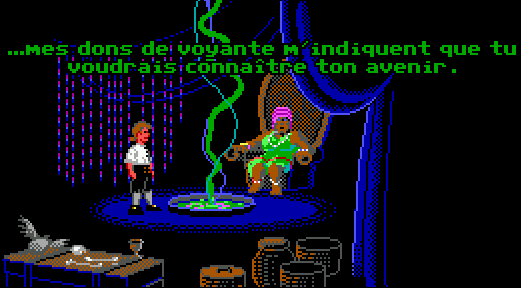
\includegraphics[width = 7cm]{images/captureMI.png}
\end{center}
}

\paragraph{Ton personnage}
{
Oui~!  Tu le vois.
Il va vers la Tour et il y rencontre deux autres âmes.
Tu regardes les fils associés.
Il y en a deux~:  l’un vibre énormément comme s’il essayait de se libérer d’une frontière invisible, l’autre possède des parties très lisses et immobiles et d’autres agitées remplies de nœuds.
Avec beaucoup de concentration, tu reconnais la Princesse de Coupes et le Gardien de la Tour.

Bon, mais tout cela ne t’avance pas beaucoup~:  le Roi va rencontrer la Princesse et le Gardien.
Tu pioches un autre Arcane et découvre la Force, à l’envers, comme si un des trois protagoniste était en colère.
Ce doit être une colère très contenue alors, ces trois personnes ont toujours été très calmes.

Bon, tout cela ne t’aide pas.
C’est bien beau de voir l’avenir, encore faut-il regarder au bon endroit…
Et il semblerait que tu ne puisses rien savoir sur ton propre sort, comme si les dieux ne voulait pas que tu le saches…
Remarque, cela signifie peut-être que tu as quelque chose à y jouer et que donc ton avenir y est très incertain.

Bon, au lieu de penser à l’avenir, essaie donc de mettre au clair le passé.
Tu étais chez la Reine blanche (tu voyages beaucoup, comme tous les autres membres de ta profession) lorsque tu prédisais la chute prochaine du Royaume de Coupes.
La Reine blanche avait l’air très préoccupée par la déclaration d’indépendance de son ancienne province et les cartes avaient parlé contre les Coupes.
La Reine semblait intéressée par ta prédiction mais pas satisfaite.
Elle t’a alors regardé droit dans les yeux et elle t’a expliqué d’une manière très calme, mais très froide en même temps, que bon nombre de gens au Royaume de Coupes croient en tes prédictions, ce qui te donnerait potentiellement un pouvoir non négligeable.
Elle t’a ensuite demandé de forcer le Destin.
Forcer le Destin~?  Le \emph{Destin}~?
Tu as beau eu l’expliquer que cela n’est pas possible, et que d’autre part tu n’as jamais menti vis-à-vis de tes prédictions et que ce n’est pas aujourd’hui que tu commenceras.
Elle t’a alors glacée par son regard.
Tu as alors compris ce qui se passerait si tu ne faisais pas ce qu’elle demandait…  Tu en frissonnes encore.

Bigre, cessons de remuer le couteau dans la plaie.
Il faut donc que tu forces les choses de façon à accélérer cette fichue prédiction.
Tu as eu beau demander aux cartes, elles ne t’ont jamais éclairé sur ton propre destin à partir de ce jour là…

De plus, ce qu’elle pense de ton prétendu «~pouvoir~» est totalement faux~:  le Fol n’a jamais cru en tes prédictions — t’accusant de charlatanerie~!
De plus, tu l’as vu, il a l’intention de se créer des fidèles parmi la cour.
Il va absolument falloir le contrer…  Mais tu as l’impression que les forces en question sont trop grandes pour toi~!
Pourtant si ton avenir est incertain, c’est qu’il est possible que tu puisses les changer.  Mais comment~?

C’est d’ailleurs assez contradictoire, mais les Arcanes semblent vibrer plus ici que dans le Royaume blanc.
Logiquement, le Royaume blanc est le lieu de créatures magiques de toutes sortes et devrait donc réagir beaucoup mieux aux cartes, mais ce n’est pas le cas.
Comme si les Arcanes voulaient tous venir ici.
Ce serait incongru et totalement absurde~!
Cela signifierait que les Arcanes, les dieux eux mêmes, refuseraient de s’intéresser à un autre endroit que celui-ci, comme si tout le reste était en train de s’effacer et de disparaître.

Et puis il y a ce monstre~!
Ce monstre porte-malheur~!
Le sournois, cruel, irascible et néfaste rongeur.
Il atteint sa victime à 100 toises, c’est un tueur.
Tel celui de la Caverne de Caerbannog, il ne fera qu’une bouchée de nous.
Ses dents sont acérées, il bondit~!
Oui, le \emph{Lapin blanc}~!

Il faut toujours ce méfier de ce genre d’animaux, et celui-ci cache quelque chose, c’est sûr.
C’est d’ailleurs la Reine blanche qui l’a amené ici.
C’est peut-être lui qui tire les ficelles derrière la Reine, lui qui te veux du mal, tu le sais.

Heureusement, certaines personnes sont raisonnables.
Il arrive même que le Roi lui-même te demande conseil.
Lui au moins considère que tes conseils valent quelque chose, qu’écouter les Arcanes chanter n’a rien de la charlatanerie~!
Et puis il y a le Gardien de la Tour aussi.
Quelqu’un de très mystérieux en fin de compte.
Tu ne penses pas l’avoir totalement cerné.
Tout ce que tu sais est qu’il a l’air de faire une confiance absolue dans tes prédictions, et tu l’apprécie beaucoup pour cela (même s’il a l’air d’avoir plus confiance en toi que toi même parfois~:  les chants des Arcanes sont parfois très complexes à comprendre).

Le concours qu’a organisé le Roi a amené beaucoup de monde.
Curieuse, tu as tenté de sonder le devenir.
Il semblerait qu’il y ait beaucoup de choses~:  les cartes ne voulaient plus se mélanger et une carte est tombée lorsque tu as coupé le jeu~:  l’Hermite.
Seul hic~:  il n’est pas tombé dans un sens précis (il était de côté).
Est-ce un conspirateur~?  Un mage~?
Tout ce que tu sais est qu’il y a quelqu’un de puissant dans les spectateurs… de très puissant.

Bon, tes pensées s’égarent~!
Il faut que tu trouves un moyen pour faire chuter ce fichu Royaume…  Surtout que la Reine arrive bientôt~!
Elle semble n’avoir prévenu personne, mais elle va arriver très bientôt.

Tu regardes par la fenêtre et t’aperçois alors que le Roi est en train de discuter avec la Princesse et le Gardien.
Et voilà, tu as réfléchi tellement longtemps que le futur est devenu présent~!

Bon, il est temps d’observer ce que font les gens, et de réfléchir à ce que tu pourrais bien faire pour renverser le royaume… ou fuir la Reine~!
}

\paragraph{Les prédictions}{
La Voyante va probablement être consultée plusieurs fois durant la partie.
Il faudra alors tirer les cartes (si la Voyante daigne accepter de se pencher sur la question avec ses cartes bien entendu) et en tirer une interprétation.
Dans ces cas là, merci de prévenir un des maîtres du jeu (ou de rapporter l’interprétation et le tirage — au moins la première et la dernière carte).
Il faut bien que ces derniers soient au courant de la volonté divine~!

Je tiens à préciser que les premières fois que l’on essaie de prédire l’avenir, ça ne paraît jamais plausible.
Au bout de quelques prédictions, on finit par broder autour des cartes…  Il faut juste s’entraîner deux ou trois fois avant la partie~!
}

\mj{
\paragraph{Note aux MJ}{
Ce personnage n’est pas des plus simple~:  il faut non seulement être capable d’inventer une interprétation plausible du tirage, mais en plus être capable de la modifier en fonction de ce qui nous arrange.
Une autre difficulté (mais qui fait la force du personnage) et d’interpréter les questions des joueurs~:  la plupart des joueurs vont vouloir «~crypter~» leurs questions afin de ne pas trop donner d’informations à la Voyante.
En regardant les réactions des joueurs, on peut arriver à extraire de grandes informations.

Tout ça pour dire que ce personnage est plutôt réservé aux joueurs avancés (ou aux cartomanceurs, mais je doute que ça soit si fréquent \Smiley).
}
}

\citations{
	\item Ainsi, tu oserais te battre contre une femme~?
	\item N’oublie pas que je vois l’avenir~:  pourquoi aurais-je accepté le combat si je ne le gagnais pas~?
	\item Crois-tu que les les dieux verront d’un bon œil la défaite de leur messager~?
}
}

\player{10}{
\section{Ton personnage~:  L’Inconnu}

\paragraph{Description physique}
{
Ce personnage est assez spécial puisque son apparence dépend fortement de la personne qui le regarde.
Au début, il ressemblera à un sujet normal du Royaume de Coupes, mais cette apparence est amenée à changer…
}

\paragraph{Ton personnage}
{
La réalité commence déjà à s’effondrer.
Le Monde s’affaiblit tandis que la Tempérance et l’Arcane sans nom deviennent de plus en plus importants.

Tu étais là lorsque ce monde a été créé.
C’est d’ailleurs toi en parti qui l’a créé.
Sans toi, toutes les personnes ici présentes penseraient de la même manière.
Tu es le dieu de la diversité, le neuvième Arcane majeur~:  l’Hermite.

Malheureusement, la réalité t’a oublié depuis un certain temps.
Ton influence est présente dans tout le Pays des Merveilles, mais tu sens que tu es appelé par ici.
Tu n’es pas le seul Arcane majeur présent d’ailleurs.
Le Fol est ici, tu vois aussi la Tour au loin qui s’est amusée à prendre forme à la place de la bibliothèque du Roi, comme si elle cherchait à le manipuler.
Oui, si l’on t’a appelé ici, c’est bien qu’il va s’y passer quelque chose.

Tu as donc pris l’apparence d’un sujet du Roi qui va tenter de conquérir le cœur de la Princesse.

En tant qu’Arcane majeur, ton apparence et tes émotions vont changer en fonction de la personne à qui tu parles.
Par exemple du point de vue du Sage, tu représentes la réflexion profonde~:  tu apparaîtras au fur et à mesure comme quelqu’un d’extrêmement sage pour lui.
Pour toutes les personnes un peu belliqueuses, tu finiras progressivement par ressembler à une bête fabuleuse (type dragon asiatique) qu’il faudrait abattre car elle est différente.
Ta «~vraie~» nature ressemble pourtant plus à celle que verront peu à peu le Fol, la Voyante et le Gardien de la Tour (sous l’influence probable de cette dernière), qui est celle de quelqu’un exilé à cause de ses façons différentes de penser, de se comporter ou de son apparence différente.

En fait, tu es tout cela en même temps.
Tu es une abstraction vivante, une partie de ce monde.
La limite d’action entre les Arcanes n’est jamais très clair, tu fais donc tout aussi bien parti partiellement du Fol et de la Tour.

Mais tu es avant tout le dieu des exilés~:  ta tâche céleste est avant tout de les trouver et les aider.
Ils sont comme toi.  Ils sont perdus, ils ont besoin d’aide et de réconfort.
De quelqu’un qui les comprends.

Tu es une allégorie.
La notion de mort t’es inconnue, et tu n’hésiteras jamais à faire des choses qu’un simple humain n’oserait pas faire (dans le pire des cas, il te suffira de choisir une nouvelle apparence).
Cependant, si tu ne respectes pas les valeurs de l’Hermite, tu risques de te désagréger, comme une métaphore que l’on ne pourrait plus filer…
C’est le seul moyen pour toi de mourir~:  celui de ne pas respecter les valeurs du neuvième Arcane majeur (dans les deux sens de la carte bien entendu).

Tu sais que ta présence ne passera pas inaperçu, et tu sens que presque tout le monde ici a besoin de toi.
Même si le Monde ne tiendra pas longtemps face à l’Arcane sans nom, tes valeurs tiendront aussi longtemps que tu seras là.
}

\citations{
	\item À ce que je vois, tu m’as pris en passant…  Ne serais-tu qu’un simple pion~?
	\item Tu n’aurais pas dû te tremper dans cette histoire.
	\item Mon pauvre ami, être obligé de vouloir me tuer comme cela…  Tu dois vraiment être très seul.  Viens donc avec moi plutôt~!
}

\paragraph{Pouvoir spécial}{
En tant qu’Arcane majeur (i.e. divinité), tu as bien entendu le droit de modifier la réalité lorsque tu le demandes.
Il te suffira de demander aux maîtres du jeu ce que tu veux modifier.
N’oublie pas par contre d’une part que tes pouvoirs sont limités à ceux de l’Hermite, et d’autre part qu’ils semblent moins puissants par ici à cause de la dégénérescence progressive de la réalité.
Tu peux aussi tout simplement demander des renseignements~:  ta sagesse et tes connaissances sont quasi-infinies et il est très probable que tu connaisses des détails bien précis sur beaucoup de gens ici, surtout si cela est relié à un isolement quelconque de leur part.

Bon, tout cela n’empêche pas que leurs problèmes soient complexes à résoudre…  D’autant qu’il y a de très nombreuses manières d’être isolé~!
}
}

\player{11}{
\section{Ton personnage~:  L’Inventeur}

\paragraph{Description physique}
{
Assez vieux, habillé tout en blanc et bleu (blanc comme la pureté et bleu comme le symbole du Royaume de Coupes).
Il porte sur lui un exemplaire du dernier poème qu’il a composé (en l’occurrence, le \textsc{Jabberwocky} mis en annexe), de manière assez visible dans un papier roulé qu’il porte à la main.  (Il pourra bien entendu le poser quelque part lorsqu’il n’est pas en cérémonie, mais jamais le plier~:  ce serait un sacrilège~!)
}

\paragraph{Ton personnage}
{
Un concours pour trouver le meilleur poète du Royaume~?
\emph{Un concours pour trouver le meilleur poète du Royaume~!}

De qui se moque-t-on~?
Tu es le meilleur poète jamais en fonction dans ce palais et on chercherais à en trouver un meilleur~?
Tout cela en échange de quoi~?
La main de la Princesse~!

Comme si un poète voudrait gâcher ses poèmes pour les lire devant une foule qui n’y connaît rien en échange d’un de ces plaisirs terrestres~?
Un poète ne se nourrit pas de ça, bon sang~!

Alors que toi, toi qui n’a jamais demandé quelque chose en échange, toi qui a été l’auteur de la toute dernière figure de style inventée il y a quelques années, on t’oublierais, comme ça~?
Il en est hors de question~!
Tu ne te laissera pas faire, par tous les dieux~!

Oublierais-t-on à qui l’on doit l’invention du mot-valise, cette figure de style qui a tant plut au gens par le passé et qui t’a valu le titre d’\emph{Inventeur}~?
Oublierais-t-on tes milliers de poèmes composés pour satisfaire l’appétit du Roi~?
Des \emph{milliers} de poèmes, oui~!
Tout cet effort que tu as donné, pour rien~?
Tout cela pour qu’au moment où tu commences à vieillir on te jette comme une cagette usagée\footnote{
Tiens~?  Ça te donne une idée de poème ça, mais revenons à nos mouton.}~?

Tu retournes ouvrir tes anciens ouvrages.
Tu le fais à peu près tous les jours.
Cela te rappelle qui tu es vraiment~:  l’auteur de tous ces livres.
\textit{Sylvie et Bruno}, \textit{La chasse au Snark}, \textit{Le Parapluie du presbytère}…
Tu les as tous composés, écrits, d’un bout à l’autre~!
Y en a-t-il un seul parmi tous ceux qui se présentent aujourd’hui qui vaille ta gloire passée~?
Ne serais ce qu’un seul~?
Aucun, \emph{aucun}, mon ami~!
Absolument aucun~!

Ce concours n’est qu’une mascarade pour te jeter aux portes du Royaume~!
Une mascarade oui, une insulte à la poésie~!
Qui irait présenter le fruit de son dur labeur à une foule si ignorante~?
Certainement pas un poète en tout cas~!
Un poète vit dans la cour du Roi~!
Il n’y a que là où l’on puisse trouver un véritable poète.
Les autres sont piégés par les vérités de survie terrestre.
Ne le voyez vous donc pas mon Roi~?

Mais non, il ne peux pas le voir.
Il veut se débarrasser de toi, définitivement.
Quel ignorant~!
Que dis-je, quel ignare~!

Il ne te reste décidément qu’un seul moyen, qu’une seule voie, qu’un seul passage~:
il faut que tu sabotes le concours.
Si tu commences à faire un scandale, ce sera finit de toi.
Il faut donc que tu fasses comme si tu acceptais ce concours comme tout ordre du Roi.
Mais il faut que tu trouves un moyen — qui ne permettra pas de remonter à toi — de saboter ce concours.
N’importe quel moyen suffira~!

Qu’un concurrent fasse un scandale, devienne fou ou se mette à menacer de mort certaines personnes bien placées.
Que la Princesse soit enlevée ou annonce qu’elle refuse ce concours.
Qu’une armée ennemie attaque le Royaume~!
Qu’un tremblement de terre arrive~!
\emph{Que les dieux attaquent le Royaume~!}
N’importe quoi fera l’affaire.

\begin{verse}
Or, comme il ruminait de suffêches pensées, \\
Le Jabberwock, l’œil flamboyant, \\
Ruginiflant par le bois touffeté, \\
Arrivait en barigoulant.
\end{verse}

Un tel monstre serait parfait…
Dommage que ce ne soit qu’une image sortie de ton génie.

Peut-être que la Voyante pourrait t’aider à influencer certaines personnes un peu folles~?  Hum…  Elle te demanderait quelque chose en échange, elle n’est pas si serviable.
Un moyen serais de composer un poème en l’honneur de ses Arcanes~:  cela pourrait l’aider à obtenir une meilleur place dans pour le Roi.
Mais comment le Sage pourrait-il accepter cela~?  Tu poignarderais ton amis~?
Ma foi, tu n’es pas sûr d’avoir vraiment le choix.
Entre le Sage et la Voyante, il va falloir faire un choix.  Le plus important pour toi est de garder ta place.

Peut-être faire confiance au Sage serait pour une fois une bonne idée, il faudra juste se méfier à ne pas attirer l’attention du Roi sur toi dès le début.
Tu te diriges donc vers le Sage pour lui demander conseil.
}

\paragraph{Pouvoir spécial}{
En tant que poète, tu as l’inspiration facile.
N’hésites donc pas à demander aux maîtres du jeu des poèmes tout fait au cours de la partie.
}

\citations{
	\item Ma langue est plus pointue que n’importe quelle épée.
	\item Mon pauvre, tu fais honte à ta race et à tes glorieux ascendants~!
	\item Qu’est-ce qui t’impressionne le plus en moi, freluquet~?
	\item \begin{verse}
		Un jour, tu regretteras cet affront~! \\
		Tu verras alors que tu n’as absolument aucun don, \\
		Que les dieux t’abandonnent comme un gros…
	\end{verse}
}
}

\player{12}{
\section{Ton personnage~:  Le Lapin blanc}

\paragraph{Description physique}
{
C’est un lapin blanc.
Il est tout petit, mais vraiment trop mignon~!
}

\paragraph{Ton personnage}
{
Tiens~?  Une carotte~!
Non, ce n’est pas raisonnable ça…  N’oublie pas que tu es en pleine mission~!

S’il y a bien une chose qui n’a pas changé depuis tout ce temps, c’est ton affection pour les carottes.
(Et puis bien entendu ta peur des chats, surtout lorsqu’ils sont noirs.)

Pourtant, il y en a des choses qui ont changé entre-temps~!
Tu te souviens encore des horreurs qui se sont produites lorsque la Reine de Cœur était au pouvoir et que tu étais son valet.
À l’époque, personne ne connaissait ton vrai nom, \textsc{Eusèbe}.
Bon, maintenant, les hommes continuent de t’appeler \emph{le Lapin blanc}, mais au moins certains connaissent ton nom.

À cette époque, le monde n’était pas spécialement sympathique, en partie à cause de la Reine Rouge, mais surtout à cause du Royaume de Cœur en fait.
Heureusement un jour la Reine blanche est arrivée et t’a sauvé.
Tu lui fais maintenant entièrement confiance.

Lorsque tu as appris que l’ancienne province de Coupes, qui se trouve à l’emplacement de l’ancien Royaume de Cœur, avait fait sécession, tu t’étais tout de suite présenté comme volontaire pour être un agent de la Reine blanche là-bas.
Tu penses que la magie maléfique du Royaume de Cœur (ou de Coupes maintenant) n’a pas cessé d’exister.
La preuve d’ailleurs~:  c’est maintenant un monde de malheurs, sans aucune créature enchantée.
Uniquement des hommes~!
C’est juste impensable~!

N’oublions pas que la Reine de Cœur ainsi que toute sa cour était composé d’hommes~!
Il y a une chose cependant qui est rigolote avec les hommes~:  ils te considèrent comme tellement mignon qu’ils ne se sont jamais attaqués à toi (en tout cas pour l’instant).
Ce fait ainsi plusieurs mois que tu es en mission ici, dans le nouveau Royaume de Coupes, à espionner son système.

Ce qui t’étonne le plus, c’est que le Roi ne te semble pas agressif.
Il ne ressemble pas du tout à la Reine de Cœur, ni dans son apparence, ni dans sa façon de gouverner.
Pourtant la magie maléfique est là, tu le sais~!

Il se passe quelque chose par ici.
Tu penses avoir des soupçons particuliers pour quelqu’un d’autre néanmoins~:
le Chevalier est quelqu’un de beaucoup plus dur dans ses paroles et ses actions.
Tu penses que c’est à travers lui que la malédiction apparaît et qu’il va falloir le prouver.
Il est très porté par l’alcool, mais c’est pourtant le maître d’arme du Royaume.
Son nez ridicule te rappelle les excroissances des hommes de la cour de la Reine de Cœur.

Tu as appris qu’il sera chargé des festivités lors du concours pour marier la Princesse et tu commences à t’inquiéter à cause de ça.

Mais attends…  Tu es là depuis quelques mois…
\emph{Quelques mois~!}
Tu es en retard~!

La Reine blanche était censée arriver quelques mois après toi.
Que dira-t-elle lorsqu’elle apprendra que tu n’as rien fait~?
Il ne faut surtout pas que cela arrive~:  zut, zut, il faut absolument que tu compenses ton retard \textsc{Eusèbe}~!
Tu abandonnes la carotte et va te précipiter espionner le Chevalier, il te semble être la piste la plus probable de ce mal qui ronge le Royaume.
}

\paragraph{Pouvoir spécial}{
Malgré le fait qu’on ai tendance à le répéter, les joueurs peuvent oublier que tu es trop mignon.
Tu peux demander aux maîtres du jeu à faire tes yeux doux au Roi pour annuler un duel \textit{(à utiliser avec parcimonie cependant)}.
}

\citations{
	\item Halte-là, misérable~!  Viens donc tâter de ma lame, tueur de lapins~!
	\item Je vise juste et ma vigilance est sans faille.
	\item S’attaquer à un tout petit lapin sans défense.
		C’est bien bas que les hommes sont tombés.
}
}

\player{13}{
\section{Ton personnage~:  Armand Raynal de \textsc{Maupertuis}}

\paragraph{Description physique}
{
Habillé comme les nobles de ce Royaume (i.e. avec une composante de bleu relativement dominante).
Il porte sur lui une épée d’escrime.
}

\paragraph{Ton personnage}
{
Tu es un noble du Royaume de Coupes.
Cela ne fait pas de toi quelqu’un de très connu, mais tu es tout de même important~:
que ferait un Royaume sans ses nobles~?
Ce sont eux qui le défendent lorsqu’il en a besoin.

Tu es tout à fait prêt à donner ta vie pour le Royaume.
Sinon, à quoi bon être noble~?
La noblesse passe avant tout par l’honneur.

S’il y a bien une chose chez toi qui est bien inébranlable par \textsc{Maupertuis}, c’est bien ton sens de l’honneur.
Tu ne te bats pas très bien, tu le sais, mais tu donnerais ta vie sans réfléchir pour le Royaume.
Ce Royaume si bien gouverné par un Roi plein de goût et de finesse.

Tu as toujours voulu parler de poésie avec lui.
Il a vraiment l’air d’un souverain cultivé et sage et tu es fier d’être un noble de ses contrées.

L’honneur te dicte d’ailleurs de nombreuses choses.
Jamais tu n’irais te vanter de quoi que ce soit, mentir ou refuser d’aider une personne qui te le demande.
Tu prends ces codes très au sérieux car tu sais que sans cela, le système ne pourra jamais tenir.

Lorsque tu as entendu parlé du concours organisé par le Roi, tu t’es tout de suite dit que c’était l’occasion ou jamais de parler poésie avec ce superbe souverain.
Tu t’es donc empressé d’y participer.
Mais tu y va dans un but totalement désintéressé~:  tu sais que tu n’as pas le niveau pour sortir vainqueur de cet évènement, tu n’y vas que pour pouvoir t’exercer en poésie avec les autres sujets du Royaume.

Lorsque tu es arrivé sur la place, tu étais en trance.
Tous ces gens arrivés ici pour parler poésie, c’était magnifique.
Cependant, certains points t’ont un peu déçu~:  d’un côté certains étaient presque tombés dans des extrêmes comme le Fol qui accordait tellement d’importance à la poésie qu’il en oubliait le monde réel (et comment peut-on vivre en dehors de ce monde comme cela~?  Il faut raisonner cet homme~!), et de l’autre des gens dont l’équilibre poétique est proche de zéro.
Tu penses notamment pour illustrer le second point le pourtant célèbre Chevalier de Coupes.
D’après les récits que tu avais lu, il est un homme d’honneur plein de bravoure et de charme.
Lorsque tu l’as aperçu, tu n’y as vu qu’un ivrogne sombrant dans la vanité…
Et c’est lui qui est censé faire régner la sécurité lors du concours~?  Non, cela n’a pas de sens.
Tu as donc décidé de mener en parallèle une surveillance du concours — tu n’as pas vraiment confiance en cette personne, et il est de ton devoir de noble de compenser cela en protégeant les honnêtes gens présents ici.
D’après l’agitation anormale des gens, il semblerait qu’il y ai quelques affaires complexes qui se déroulent par ici (mais tu n’as pas pu comprendre de quoi il s’agissait).
Il est de ton devoir de comprendre tout ce qui s’y déroule, par \textsc{Maupertuis}~!

Tu as alors aperçu la femme que tout le monde appelait la Reine blanche.
Tu as alors presque oublié ces menus problèmes — bien que tu n’ai pas oublié de prévenir le Roi de ces événements pour le moins douteux…
La \emph{Reine blanche}.
Tu es tout de suite tombé sous ses charmes, les traits de Cupidon ne t’épargnant aucunement.
Tu ne vois pas ce qui pourrait t’arrêter maintenant.

Tu serais prêt à remuer terre et ciel pour qu’elle daigne t’accorder une part de son temps.
Tu sais maintenant quel sera l’objet de tous les poèmes que tu composera sur cette place~:
ils seront tous pour la femme de tes rêves~!

Et ils seront magnifiques, car l’amour ne peut que répandre beauté dans ce monde d’ici bas~!
Le Roi ne pourra que donner sa bénédiction à une telle union.
Le royaume du bleu et du blanc, tel le ciel et ses nuages.
C’est cela~!  Tu espères faire entrer la Reine blanche dans tes rêves nébuleux et célestes.
Que le Royaume blanc devienne de Coupes et celui de Coupes devienne blanc par cette future union bénite par ton amour céleste~!

Et qu’importe si elle ne te désire pas, elle sera alors ta Dulcinée et tu feras tout ce qu’elle te demande~!
Une dame d’une telle beauté doit-être d’une noblesse sans faille et tu es tout impatient de la connaître.
Même dans cette situation de tragédie, l’Amour et l’honneur seront tes maîtres mots.

\textit{Je suis enivré, madame, du plus doux des spiritueux~: votre beauté~!}
}

\citations{
	\item \textsc{Maupertuis} Ose et Rit~! \\
		(Contre-parade possible\footnote{
	Cela signifie qu’il est possible pour toi de contre-attaquer la réplique de quelqu’un par cette réplique.
	Attention à bien vérifier que cette contre-attaque ai vraiment un sens dans le contexte~!
}~:  «~C’est grotesque~!  Cette devise, monsieur, glapie par ma famille depuis \textsc{Azincourt}, n'a rien de risible~!~»)
	\item Fois de \textsc{Maupertuis} — lame en avant, jambes fléchies — par mon regard vif et ardent, je t’occis~!
	\item \begin{verse}
			Monseigneur, très intimement je crois, \\
			Qu’un jour de gloire l’absolu Honneur \\
			Sans aucun doute possible triomphera \\
			Je crains que vous aurez alors bien peur.
		\end{verse}
}
}

\player{11}{
\newpage

\section{Annexe~:  le \textsc{Jabberwocky}}
\begin{flushright}
\small
Je modifie l’espacement sur la page pour faciliter la découpe du poème, j’espère vous m’excuserez de cette mise en page pourrie.
\end{flushright}

\begin{center}%
\makebox[0.4\textwidth]{%
\leaders\hbox{\Cutline}\hfill%
}%
\Cutright%
\makebox[0.4\textwidth]{%
\leaders\hbox{\Cutline}\hfill%
}%
\end{center}

\vspace{1.5cm}

\begin{verse}
Il était grilheure ; les slictueux toves \\
Gyraient sur l'alloinde et vriblaient~: \\
Tout flivoreux allaient les borogoves ; \\
Les verchons fourgus bourniflaient. \\
~\\
«~Prends garde au Jabberwock, mon fils~! \\
A sa gueule qui mord, à ses griffes qui happent~! \\
Gare l'oiseau Jubjube, et laisse \\
En paix le frumieux Bandersnatch~!~» \\
~\\
Le jeune homme, ayant pris sa vorpaline épée, \\
Cherchait longtemps l'ennemi manziquais… \\
Puis, arrivé près de l'Arbre Tépé, \\
Pour réfléchir un instant s'arrêtait. \\
~\\
Or, comme il ruminait de suffêches pensées, \\
Le Jabberwock, l'oeil flamboyant, \\
Ruginiflant par le bois touffeté, \\
Arrivait en barigoulant. \\
~\\
Une, deux! Une, deux! D'outre en outre~! \\
Le glaive vorpalin virevolte, flac-vlan~! \\
Il terrasse le monstre, et, brandissant sa tête, \\
Il s'en retourne galomphant. \\
~\\
«~Tu as donc tué le Jabberwock~! \\
Dans mes bras, mon fils rayonnois~! \\
Ô jour frabieux~! Callouh~! Callock~!~» \\
Le vieux glouffait de joie. \\
~\\
Il était grilheure ; les slictueux toves \\
Gyraient sur l'alloinde et vriblaient~: \\
Tout flivoreux allaient les borogoves ; \\
Les verchons fourgus bourniflaient.
\end{verse}

\vspace{1cm}

Henri \textsc{Parisot}, traduit de Lewis \textsc{Carroll} — aussi nommé ici l’\textit{Inventeur}.
}

\end{document}

